\documentclass[12pt,a4paper]{article}
\usepackage[T1]{fontenc}
\usepackage[utf8]{inputenc}
\usepackage[ngerman,english]{babel}
\usepackage{lmodern,microtype}
\usepackage{csquotes}
\usepackage{amsmath,amssymb}
\usepackage{booktabs,array,longtable}
\usepackage{graphicx}
\usepackage[numbers,sort&compress]{natbib}
\usepackage[hidelinks]{hyperref}
\graphicspath{{figures/}}
\setlength{\parindent}{0pt}
\setlength{\parskip}{0.8em}
\setlength{\emergencystretch}{3em}
\renewcommand{\topfraction}{0.9}
\renewcommand{\textfraction}{0.05}
\renewcommand{\floatpagefraction}{0.85}
\renewcommand{\arraystretch}{1.12}
\newcommand{\SO}{\mathrm{SO}(3)}
\newcommand{\SE}{\mathrm{SE}(3)}
\newcommand{\crossmat}[1]{[#1]_{\times}}
\newcommand{\code}[1]{\texttt{\detokenize{#1}}}
\widowpenalty=10000
\clubpenalty=10000

\begin{document}
\pagenumbering{gobble}
\begin{titlepage}
\centering
\begin{flushright}

\includegraphics[width=0.5\linewidth]{Logo-Hochschule-Darmstadt.png}
\end{flushright}
\vspace{1.5cm}
{\large\bfseries Bachelor's Thesis\\Bachelor's program in Applied Mathematics\par}
\vspace{1.5cm}
{\huge\bfseries Experimental Comparison of Hand--Eye Calibration Methods for a Laboratory Robot\par}
\vspace{2cm}
{\Large Yana Osinchuk\par}
\vspace{1cm}
{\Large October 2026\par}
\vfill
\begin{flushleft}
Supervisor\\Prof.\ Dr.\ Thomas Maerz
\end{flushleft}
\end{titlepage}
\pagenumbering{roman}

\section*{Declaration}
\addcontentsline{toc}{section}{Declaration}
I affirm that I have independently authored this document and have not used sources or aids other than those explicitly mentioned. Any directly quoted or paraphrased passages from other works are appropriately acknowledged.
\vspace{2cm}

Yana Osinchuk

\clearpage
\section*{Summary}
\addcontentsline{toc}{section}{Summary}
This thesis compares the five hand--eye calibration methods implemented in OpenCV 4.12.0: Tsai--Lenz, Park--Martin, Horaud--Dornaika, Andreff--Horaud--Espiau and Daniilidis. The theoretical discussion is restricted to their formulations and implementation differences. The experiments use a fixed camera and a target attached to the robot's tool frame. Robot poses are inverted before calling OpenCV's standard hand--eye interface. \cite{opencv,opencvsource}

Two controlled synthetic models perturb either complete poses or image coordinates followed by perspective-n-point estimation. They vary acquisition count, orientation diversity and noise, using 100 seeded trials per condition. A further simulation projects the target along 20 recorded DENSO robot poses. Together these comparisons contain 33,000 synthetic method attempts. Real-image validation fits the complete calibration chain on all but one observation and predicts each of 15 June and 18 July images, giving 165 method-specific held-out predictions. All published condition summaries were reproduced with the pinned numerical dependencies. \cite{experimentcode}

At 20 poses and low noise in the trajectory replay, Daniilidis gives a median translation error of 0.962 mm. It also gives the smallest median held-out pixel RMSE in the June and July series, at 0.571 px and 1.662 px. These observations do not establish a universal ranking: the controlled nearly single-axis experiments expose large translation tails, including finite but extremely inaccurate Daniilidis estimates. Laboratory scores describe prediction consistency; no independently surveyed camera pose is available. The circular-target diagnostic supports image/robot correspondence by pose identifier but does not validate the full circular-target hand--eye transform. \cite{experimentcode,eauncertainty}

\clearpage
\begin{otherlanguage}{ngerman}
\section*{Zusammenfassung}
\addcontentsline{toc}{section}{Zusammenfassung}
Diese Bachelorarbeit vergleicht die f\"unf in OpenCV 4.12.0 implementierten Verfahren der Hand-Auge-Kalibrierung: Tsai--Lenz, Park--Martin, Horaud--Dornaika, Andreff--Horaud--Espiau und Daniilidis. Die theoretische Darstellung beschr\"ankt sich auf ihre Formulierungen und Implementierungsunterschiede. In den Experimenten ist die Kamera fest montiert, w\"ahrend die Kalibriertafel am Werkzeugkoordinatensystem des Roboters befestigt ist. Vor dem Aufruf der OpenCV-Schnittstelle werden die Roboterposen invertiert. \cite{opencv,opencvsource}

Zwei kontrollierte synthetische Modelle st\"oren entweder vollst\"andige Posen oder Bildkoordinaten mit anschlie\ss ender Perspective-n-Point-Sch\"atzung. Untersucht werden die Anzahl der Aufnahmen, die Vielfalt der Orientierungen und das Messrauschen mit jeweils 100 reproduzierbaren Zufallsversuchen pro Bedingung. Eine weitere Simulation projiziert die Tafel entlang von 20 aufgezeichneten DENSO-Roboterposen. Insgesamt ergeben sich 33\,000 synthetische Verfahrensauswertungen. Die Validierung realer Bilder sch\"atzt die gesamte Kalibrierungskette jeweils ohne eine Beobachtung und sagt jedes der 15 Juni- und 18 Julibilder voraus. Dies ergibt 165 verfahrensspezifische Validierungsvorhersagen. Alle ver\"offentlichten Bedingungszusammenfassungen wurden mit den festgelegten numerischen Abh\"angigkeiten reproduziert. \cite{experimentcode}

Bei 20 Posen und geringem Rauschen erreicht Daniilidis in der Trajektoriensimulation einen medianen Translationsfehler von 0,962 mm. Das Verfahren liefert auch die kleinste mediane Pixel-RMSE der zur\"uckgehaltenen Juni- und Julibilder mit 0,571 px beziehungsweise 1,662 px. Daraus folgt keine allgemeing\"ultige Rangfolge: Die kontrollierten Versuche mit nahezu einachsigen Bewegungen zeigen gro\ss e Translationsfehler in den Verteilungsr\"andern, einschlie\ss lich endlicher, aber extrem ungenauer Daniilidis-Sch\"atzungen. Die Laborwerte beschreiben die Konsistenz der Vorhersagen; eine unabh\"angig vermessene Kamerapose liegt nicht vor. Die Diagnose der Kreistafel unterst\"utzt eine Zuordnung \"uber Posenkennungen, validiert jedoch nicht die vollst\"andige Hand-Auge-Transformation dieser Tafel. \cite{experimentcode,eauncertainty}
\end{otherlanguage}

\clearpage
\section*{Preface}
\addcontentsline{toc}{section}{Preface}
I would like to thank Prof. Dr. Thomas Maerz from the bottom of my heart for everything he has done for me. Throughout my studies, he has given his time, advice, and encouragement so generously. His continued willingness to help has meant more to me than I can fully express here.

I am especially grateful for his help in finding my internship at the Hessian Agency for Nature Conservation, Environment and Geology (HLNUG), and for arranging an opportunity for me to work in the robotics laboratory. He also spoke with another professor to obtain the necessary permission for my work there. Each of these steps required his time and effort, and each made a real difference to my education and the opportunities available to me.

What I appreciate most is the kindness and care behind his support. He has taken my questions seriously, and made the effort to find solutions whenever difficulties arose. Knowing that I could turn to him has given me confidence to pursue new challenges and develop my own ideas. I am deeply grateful for his trust in me, for his encouragement, and for the many opportunities he has helped make possible.

\clearpage
\tableofcontents
\clearpage
\pagenumbering{arabic}

\clearpage
\section{Introduction}\label{sec:introduction}
\subsection{Motivation}
The guiding analogy of this thesis is that hearing is not the same as listening, just as capturing an image is not the same as understanding what it shows. In \emph{Vision}, David Marr describes seeing as \enquote{to know what is where by looking}. \cite{marr2010} For a robot, the question of where an object is has a practical consequence: its location must be expressed in coordinates that the robot can use to plan and execute a movement. This requires a geometric connection between the camera's observations and the robot's description of space.

A robot and a camera describe the same physical world using different coordinate systems. The robot controller reports the position and orientation of the end effector relative to the robot base. A camera observes image features and, when a target of known geometry is visible, can estimate the target's position and orientation relative to the camera. Hand--eye calibration connects these descriptions. In the eye-to-hand arrangement investigated here, the camera is fixed relative to the base and the target is attached to the robot's tool frame. The classical equation $AX=XB$ expresses compatible relative motions and an unknown fixed transformation. \cite{tsai,halconde,wenhardtde}

The practical difficulty is that the observations are imperfect. Image measurements, camera calibration, robot pose uncertainty and the distribution of acquisition poses affect the estimated relationship. The selected solvers use different algebraic representations and numerical procedures. Comparing their behaviour therefore requires shared observations, a clear experimental protocol and evaluation criteria that distinguish known-reference error from prediction consistency. \cite{eauncertainty,opencvsource}

\subsection{Objective and Research Question}
This thesis compares the five methods provided by OpenCV's hand--eye calibration interface: Tsai--Lenz, Park--Martin, Horaud--Dornaika, Andreff--Horaud--Espiau and Daniilidis. The laboratory robot-camera installation provides the practical setting. The central research question is:
\begin{quote}
How do the five OpenCV hand--eye calibration methods differ in validation performance and repeatability for the laboratory installation, and how do the number and diversity of calibration poses affect these differences?
\end{quote}
The evaluated objects are the particular implementations in OpenCV 4.12.0. Their mathematical formulations form the theoretical framework in Section~\ref{sec:methods}. \cite{opencv,opencvsource}

The completed work addresses the question using controlled pose and pixel simulations, a simulation on recorded DENSO motions, and leave-one-pose-out prediction of laboratory images. Repeated numerical trials and shared subsets quantify sensitivity to the selected perturbations and observations. Independent repeated physical acquisitions were not performed, so physical repeatability is not established by these results. \cite{experimentcode,eauncertainty}

\subsection{Scope and Contribution}
The contribution is a reproducible comparison that links a focused account of the five solver formulations to their implemented observation models and experimental results. All methods receive the same observations within each trial. Camera intrinsic calibration and image-based target-pose estimation are treated as documented upstream stages of the laboratory prediction chain. \cite{experimentcode,halconde}

Accuracy is assessed through agreement with a known or independently measured reference. Consistency describes agreement with additional observations. Repeatability concerns variation under specified repeated-acquisition conditions. Synthetic data provide a known numerical reference; the available laboratory archive supports held-out consistency evaluation but contains no independently surveyed camera pose. No solver is assumed to be universally superior. \cite{eauncertainty,experimentcode}

\subsection{Structure and Reading Guide}
Section~\ref{sec:methods} provides the theoretical framework for the five methods. Sections~\ref{sec:simulation} and~\ref{sec:laboratory} describe the synthetic models, laboratory processing and validation. Section~\ref{sec:results} presents the results, followed by the conclusions in Section~\ref{sec:conclusion}. The appendices contain the implementation inventory, complete numerical summaries, data corrections and reproduction commands.

\clearpage
\section{Theoretical Framework}\label{sec:methods}
The study asks how the five OpenCV implementations differ under shared observations, controlled perturbations and held-out image prediction. The theoretical scope is limited to these methods. Their common algebraic problem is
\begin{equation}\label{eq:axxb}
A_\ell X=XB_\ell,
\qquad
(R_{A_\ell}-I)t_X=R_Xt_{B_\ell}-t_{A_\ell},
\end{equation}
where $A_\ell,B_\ell$ are corresponding relative motions. Here $X$ denotes a generic unknown; in the implemented eye-to-hand experiments that unknown is the camera-to-base transform $Y$ defined in Section~\ref{sec:simulation}. Tsai, Park and Horaud estimate rotation before translation; Andreff and Daniilidis couple the two parts. All five are called through \code{cv2.calibrateHandEye}. The implementation statements below refer to the OpenCV 4.12.0 source, rather than assuming that a method name specifies every numerical detail. \cite{opencv,opencvsource}

\subsection{Tsai--Lenz}
Let $q_A=(a_0,a)$ and $q_B=(b_0,b)$ represent corresponding relative rotations. With compatible quaternion signs, the Tsai construction estimates the three-vector $u=q_{X,v}/q_{X,0}$ from
\begin{equation}\label{eq:tsai}
\crossmat{P_A+P_B}u=P_B-P_A,
\qquad P_A=2a,\quad P_B=2b,
\qquad q_X=\frac{(1,u)}{\sqrt{1+u^\top u}}.
\end{equation}
The rotation is recovered from $q_X$, and translation is fitted from the stacked equations in~\eqref{eq:axxb}. The parametrisation is singular for a hand--eye rotation of exactly $180^\circ$. OpenCV rejects a relative pair when either quaternion-vector norm is below 0.3 or above 1.7, corresponding to principal angles of approximately $17.3^\circ$ and $116.4^\circ$. Only retained pairs enter its translation solve. With fewer than two retained pairs, the routine logs a failure and can return its initial identity output. This behaviour is relevant to the narrow-orientation experiment. \cite{tsai,opencvsource}

\subsection{Park--Martin}
Park and Martin use rotation logarithms. With $a_\ell=(\log R_{A_\ell})^\vee$ and $b_\ell=(\log R_{B_\ell})^\vee$, compatible rotations satisfy
\begin{equation}\label{eq:park}
a_\ell=R_Xb_\ell.
\end{equation}
The rotational problem aligns these vector collections. The OpenCV routine forms $M=\sum_\ell b_\ell a_\ell^\top$ and evaluates $(M^\top M)^{-1/2}M^\top$ through an eigendecomposition. Translation is subsequently fitted using~\eqref{eq:axxb}. Very small eigenvalues can make this inverse-square-root calculation unstable, and a returned matrix must still be checked for a proper rotation. \cite{park,opencvsource}

\subsection{Horaud--Dornaika}
The separable OpenCV implementation expresses quaternion multiplication through left and right multiplication matrices, $L$ and $\mathcal R$. It estimates a unit quaternion by
\begin{equation}\label{eq:horaud}
\widehat q_X=\mathop{\arg\min}_{\|q\|=1}
\sum_\ell\left\|\left(L(q_{A_\ell})-\mathcal R(q_{B_\ell})\right)q\right\|^2.
\end{equation}
The smallest eigenvector of the associated symmetric matrix gives the rotation quaternion. Translation is then solved separately. The construction avoids dividing by the unknown quaternion's scalar part, although consistent signs and informative rotations remain important. The comparison evaluates this OpenCV routine, rather than all nonlinear procedures discussed in the original paper. \cite{horaud,opencvsource}

\subsection{Andreff--Horaud--Espiau}
OpenCV uses a joint linear system with nine rotation entries and three translation entries. For row-wise vectorisation $r=\operatorname{rvec}(R_X)$, a relative pair contributes
\begin{equation}\label{eq:andreff}
\begin{pmatrix}
I_9-R_A\otimes R_B&0\\
I_3\otimes t_B^\top&I_3-R_A
\end{pmatrix}
\begin{pmatrix}r\\t_X\end{pmatrix}
=
\begin{pmatrix}0\\t_A\end{pmatrix}.
\end{equation}
The stacked system is solved by least squares. The raw rotation is normalised using determinant scaling and an SVD projection, while the translation from the joint solve is retained. Rotation residuals are dimensionless, whereas translation residuals carry length units; changing the length unit changes their relative weighting in noisy data. All experiments here use millimetres. No post-normalisation translation refit is added to the OpenCV method. \cite{andreff,opencvsource}

\subsection{Daniilidis}
A rigid pose is represented by a dual quaternion
\begin{equation}\label{eq:dual}
Q=q+\varepsilon d,\qquad
\varepsilon^2=0,\qquad
d=\tfrac12(0,t)\otimes q,\qquad
q^\top q=1,\quad q^\top d=0.
\end{equation}
The equation $Q_A\otimes Q_X=Q_X\otimes Q_B$ supplies coupled linear constraints. OpenCV constructs a six-row block per motion pair, extracts the two smallest right singular vectors and selects a combination satisfying the dual-quaternion constraints through a quadratic equation. Rotation and translation are recovered together. Degenerate motion, normalisation denominators and quadratic-root calculations can affect numerical behaviour. A finite proper transform can still be very inaccurate, so validity checks and error distributions are reported separately. \cite{daniilidis,opencvsource}

\clearpage
\section{Simulation Design and Implementation}\label{sec:simulation}
\subsection{Implemented scope and coordinate convention}
The numerical simulation models a stationary camera and a target rigidly attached to the robot's tool centre point (TCP). It represents poses, target feature coordinates and image projections; it does not model motors, joint limits, collision avoidance, robot reachability, image rasterisation or the success of detecting a rendered pattern. In the pixel model, the synthetic observations are already identified image-feature coordinates. These are explicit implementation choices in \code{benchmark.py} and \code{laboratory.py}. \cite{experimentcode}

A transform maps coordinates from its lower frame label into its upper frame label. The code uses
\begin{equation}\label{eq:loop}
G_i={}^{b}T_g^{(i)},\quad M={}^{g}T_t,\quad
Y={}^{b}T_c,\quad C_i={}^{c}T_t^{(i)},\qquad G_iM=YC_i,
\end{equation}
where $b,g,c,t$ denote base, TCP, camera and target. $M$ and $Y$ are fixed. The desired estimate is $Y$. Setting $H_i=G_i^{-1}$ gives $H_iYC_i=M$, so OpenCV receives $H_i,C_i$ and its output is interpreted as camera-to-base. The associated relative equation is $A_{ij}Y=YB_{ij}$ with $A_{ij}=G_jG_i^{-1}$ and $B_{ij}=C_jC_i^{-1}$. \cite{opencv,halconde}

The supplied lecture screenshots prescribe selecting a fixed target-to-TCP pose, choosing roughly 10--20 TCP poses, transforming target points into the robot and camera frames, projecting them, checking the sensor bounds and forming paired hand--eye observations. The implemented forward chain is
\begin{equation}\label{eq:forward}
{}^{c}\bar p_j^{(i)}=Y^{-1}G_iM\,{}^{t}\bar p_j.
\end{equation}
The replay follows this direction. The generic benchmark instead samples $C_i$ and constructs $G_i=YC_iM^{-1}$, which satisfies the same chain. A numerical cross-check on one exact 16-pose sample found a maximum point-coordinate difference of $2.85\times10^{-13}$ mm between these equivalent constructions. These checks concern the implemented geometry; the screenshots do not provide a complete independently verified hardware specification. \cite{lectureplan,experimentcode}

\subsection{Generic camera, target and acquisition profiles}
The generic experiment uses a pinhole camera with zero distortion and image size $4096\times3000$ pixels. Its intrinsic matrix is
\begin{equation}\label{eq:camera}
K=\begin{pmatrix}4379.56&0&2048\\0&4379.56&1500\\0&0&1\end{pmatrix}.
\end{equation}
The camera centre is $(300,200,1000)^\top$ mm in the base frame. Its camera-to-base rotation is a $174^\circ$ rotation about $(1,-1,0)^\top/\sqrt2$. The target-to-TCP translation is $(15,-10,85)^\top$ mm and its rotation vector is $(9,-13,18)^\top$ degrees, interpreted as one axis--angle vector, not three Euler rotations. The target contains $7\times5=35$ inner corners at 20 mm spacing, centred at the target origin. These values are simulation parameters. \cite{experimentcode}

A physical pixel pitch and a physical focal length are not inputs to this camera model. If a 12 mm focal length were additionally assumed, the chosen focal length in pixels would imply $12/4379.56\approx0.00274$ mm per pixel; this is a conditional model interpretation, not a confirmed specification of the laboratory camera. The camera in the lecture screenshot has the same centre but a different orientation: its robot-to-camera rotation is $\left(\begin{smallmatrix}0&-1&0\\-1&0&0\\0&0&-1\end{smallmatrix}\right)$ and translation $(200,300,1000)^\top$ mm. The implemented generic rotation differs from this example by $6^\circ$. Thus the published runs reproduce the geometric workflow, while a literal reproduction of every handwritten numerical parameter has not been performed. \cite{lectureplan,experimentcode}

The pose counts are 8, 16 and 32. Camera-side target origins are sampled uniformly from $[-95,95]\times[-75,75]\times[620,800]$ mm. Rotation-vector components are sampled from zero-mean normal distributions with standard deviations listed in Table~\ref{tab:profiles}; these are distribution scales, not angle limits. \cite{experimentcode}
\begin{table}[!htbp]\centering\small
\caption{Generic orientation profiles: per-component rotation-vector standard deviations in degrees.}\label{tab:profiles}
\begin{tabular}{lrrr}\toprule
Profile & $x$ & $y$ & $z$\\\midrule
Diverse & 22 & 22 & 22\\
Narrow & 4 & 4 & 4\\
Nearly single-axis & 0.5 & 0.5 & 22\\\bottomrule
\end{tabular}
\end{table}

\subsection{Pose and pixel observation models}
The pose model perturbs the robot pose and the camera-side target pose independently. Rotations remain valid through a left multiplicative perturbation; frame-origin positions receive independent additive perturbations:
\begin{equation}\label{eq:noise}
\widetilde R=\exp(\crossmat{\delta r})R,\qquad
\widetilde t=t+\delta t.
\end{equation}
Rotation and position perturbations are expressed in the destination frame. This is a model with independently perturbed origin positions, rather than a full rigid left perturbation that also rotates the translation vector. The per-component noise scales are recorded in Table~\ref{tab:noise}. \cite{experimentcode,opencv}

In the pixel model, \code{cv2.projectPoints} projects all 35 ideal points through $K$. The code checks that their camera-frame depths are positive and their ideal image coordinates satisfy $0\leq u<4096$, $0\leq v<3000$. Independent normal pixel noise is then added, and \code{cv2.solvePnP} with the iterative flag recovers a target-to-camera pose. The visibility check precedes the added pixel noise; it does not recheck the noisy coordinates. Robot poses are perturbed as in the pose model. Even the exact pixel condition includes numerical PnP estimation. \cite{opencv,experimentcode}

\begin{table}[!htbp]\centering\small
\caption{Per-component standard deviations. The generic pose model applies the spatial scales independently to robot and target poses. The pixel model and trajectory replay apply them to the robot pose and use the image-noise column for the target observation.}\label{tab:noise}
\begin{tabular}{lrrr}\toprule
Level & Rotation ($^\circ$) & Position (mm) & Image coordinate (px)\\\midrule
Exact & 0 & 0 & 0\\
Low & 0.1 & 0.5 & 0.25\\
High & 0.5 & 2 & 1\\\bottomrule
\end{tabular}
\end{table}

\subsection{Paired trials, solver validity and metrics}
Each condition uses 100 trials and seed 42. \code{SeedSequence([seed, trial])} creates the random generator. Each generic trial draws a full 32-pose pool, so the shorter pose sets are prefixes of the longer sets. The same standardised random draws are reused across profiles and noise levels, and every method receives exactly the same observations within a condition. The two generic models each contain $3\times3\times3\times100\times5=13\,500$ method attempts and 135 condition-summary rows. The numerical environment is Python 3.12, NumPy 2.2.6 and OpenCV 4.12.0. \cite{experimentcode}

The solver wrapper checks finite values, $R^\top R\approx I$ and $\det R\approx1$, using NumPy comparisons with absolute tolerance $10^{-6}$ and their default relative tolerances. It rejects an exactly identity rotation with zero translation, because this known synthetic rig has a nonidentity truth and OpenCV can return that initial value after a logged failure. The check is specific to this experiment; identity is not an invalid pose in general. Exceptions in the method-estimation loop are recorded, rather than replaced with an apparently successful estimate. Upstream observation-generation exceptions are outside that loop. \cite{opencvsource,experimentcode}

For valid estimates, the recorded errors are
\begin{align}
\Delta R&=R_\star^\top\widehat R,\\
e_R&=\frac{180}{\pi}\operatorname{atan2}\!\left(
\left\|\begin{pmatrix}\Delta R_{32}-\Delta R_{23}\\\Delta R_{13}-\Delta R_{31}\\\Delta R_{21}-\Delta R_{12}\end{pmatrix}\right\|,
\operatorname{tr}(\Delta R)-1\right),\label{eq:rotation-error}\\
e_t&=\|\widehat t-t_\star\|_2.\label{eq:translation-error}
\end{align}
The angle and translation error are reported separately in degrees and millimetres. Summaries contain the median and 95th percentile of valid estimates and the number of rejected outputs. Large finite errors remain in the distributions. A low median with a large tail or many rejected outputs is therefore interpreted cautiously. The metrics and aggregation are defined by the experiment code; agreement with an independent reference is distinguished from internal consistency. \cite{experimentcode,eauncertainty}

\clearpage
\section{Laboratory Processing and Trajectory Replay}\label{sec:laboratory}
\subsection{Archive, hardware records and data audit}
The supplied \code{Data4Osinchuk.zip} contains June and July 2024 acquisitions, robot pose tables, acquisition journals, a MATLAB orientation-conversion example and robot project files. The present paired-image analysis uses the 21 June checkerboard series and the 3 July OpenCV checkerboard series. The second June folder duplicates the images and pose table. The 9 July journal describes another setup but supplies no corresponding image series in this archive. \cite{laboratoryarchive}

\begin{table}[!htbp]\centering\small
\caption{Hardware information supported by the acquisition journals and the image files.}\label{tab:hardware}
\begin{tabular}{p{0.25\linewidth}p{0.31\linewidth}p{0.31\linewidth}}\toprule
Item & June & 3 July\\\midrule
Camera record & IDS, described as green & Balluff\\
Image size & $1280\times960$ px & $4112\times3008$ px\\
Lens record & Fujinon 9 mm, f/1.4; aperture 5.6 & Fujinon 12 mm\\
Paired checkerboard views & 15 & 20, of which 18 are scored\\
Pixel pitch & Not established for this analysis & Not established for this analysis\\\bottomrule
\end{tabular}
\end{table}
The July camera model number is not documented by the inspected journal. Image DPI metadata is not treated as sensor pixel pitch. A filename in the June archive refers to an IDS UI214x data sheet, but the experiments do not require a physical pixel-pitch assumption. The replay uses fitted intrinsics and the original image dimensions, rather than the generic synthetic camera's $K$. \cite{laboratoryarchive,experimentcode}

Eight entries in the June ODS table exceed 10,000 in magnitude. The parser divides them by 1,000, treating them as missing decimal separators. Table~\ref{tab:corrections} records every input and used value. These are explicit inferred corrections, not independent measurements. July images P47 and P48 have identical PNG bytes paired with different robot poses; both are excluded from real-image calibration and scoring. The 20 logged robot poses are retained for synthetic replay, where image observations are generated afresh. \cite{laboratoryarchive,experimentcode}

\subsection{Feature detection, camera fit and target pose}
The laboratory target contains $11\times8=88$ inner corners at 12 mm spacing. Each grayscale image is reduced to approximately one third of its original dimensions for \code{findChessboardCorners}. Detected coordinates are scaled separately in the horizontal and vertical directions back to the original image, then refined with \code{cornerSubPix} on the full-resolution image. The pose identifier determines the photograph/robot correspondence. Missing checkerboard detection currently raises an exception. \cite{experimentcode,opencv}

Robot translations are used in millimetres and robot angles in degrees are converted to $R_zR_yR_x$, following the supplied MATLAB file. \code{calibrateCamera} fits $K$, five distortion coefficients and per-image target poses from the selected views. \code{solvePnP} estimates the target pose in a further image with these intrinsics and distortion held fixed. This intrinsic calibration stage is separate from the hand--eye solver. \cite{laboratoryarchive,opencv}

A full 18-view July fit gives $f_x=3750.4753$ px, $f_y=3753.0608$ px, $c_x=2084.7054$ px and $c_y=1499.0962$ px. Its distortion coefficients are approximately $(-0.09279,0.24399,0.001827,0.0003435,-0.02623)$. Its training reprojection RMS is 0.1340 px. These values parameterise the nominal replay only; the held-out evaluation below refits the intrinsic model within every training fold. The unrounded values and nominal transforms are recorded in \code{results/thesis/geometry_metadata.json}. \cite{experimentcode}

\subsection{Fixed-mount estimate and held-out prediction}\label{sec:held-out}
For a camera estimate $\widehat Y$, each training observation implies a target-to-TCP mount
\begin{equation}\label{eq:mount}
M_i=G_i^{-1}\widehat Y C_i.
\end{equation}
Translations are averaged arithmetically. If the mean rotation is $\overline R=U\Sigma V^\top$, the code uses $U\operatorname{diag}(1,1,\det(UV^\top))V^\top$ for its proper-rotation projection. This defines the experiment's mount reference; it is not an additional optimisation of the hand--eye algorithm. \cite{experimentcode,opencvsource}

For every held-out image $i$, the intrinsic matrix, distortion, hand--eye transform and mount are fitted using the other views of the same series. There are 14 training images per June fold and 17 per July fold. The held-out robot pose predicts $\widehat C_i=\widehat Y^{-1}G_i\widehat M$. A PnP pose from the held-out feature coordinates, with training-only intrinsics, supplies a pose-space comparison. Image prediction is evaluated by
\begin{equation}\label{eq:pixelrmse}
\operatorname{RMSE}_{\rm px}=
\sqrt{\frac1{88}\sum_{j=1}^{88}
\left\|\pi(K,d,\widehat C_i,P_j)-u_{ij}\right\|_2^2},
\end{equation}
where $\pi$ is the distortion-aware projection implemented by \code{projectPoints}. This is RMS Euclidean pixel distance per corner, not RMS over 176 scalar coordinate components. \cite{experimentcode,opencv}

The held-out image contributes to scoring but not fitting. The resulting 33 views give 165 method-specific predictions. They assess consistency of the complete prediction chain; the archive has no independently surveyed camera-to-base pose. Training folds overlap, and these observations are not repeated independent acquisitions. The current real-validation loop stops on a solver exception instead of recording a per-fold failure; all 165 predictions completed in the recorded runs. \cite{experimentcode,eauncertainty}

\subsection{Simulation along the recorded DENSO trajectory}\label{sec:replay}
The replay uses all 20 logged July robot poses P40--P59. A full-data Park fit and the fixed-mount mean define nominal $Y_\star,M_\star$. Ideal target poses are constructed by $C_i=Y_\star^{-1}G_iM_\star$, and all 88 corners are projected through the fitted July camera with distortion. This makes $Y_\star$ the known truth of the constructed simulation. Its prior estimation from laboratory data does not turn it into an independently measured physical truth. \cite{experimentcode}

Each trial draws a permutation of the 20 poses and shared robot and image perturbations. The 8-, 12- and 16-pose selections are nested prefixes of this permutation; the full 20-pose selection contains the same geometry in every trial. Noise levels follow Table~\ref{tab:noise}. PnP converts the noisy image points back to target poses, and all five methods receive the same noisy observations. There are $4\times3\times100\times5=6000$ method attempts and 60 summary rows. At 20 poses with zero noise, trial permutations do not represent independent geometric acquisitions. The laboratory projection helper currently has no explicit depth/sensor-bounds rejection step. \cite{experimentcode}

\subsection{Circular-target correspondence diagnostic}\label{sec:circles}
The supplementary \code{circle_diagnostic.py} processes 11 July circular-target images at $1371\times1003$ pixels. \code{findCirclesGrid} uses an $11\times11$ symmetric grid with clustering. Nine grids are detected; P43 and P54 are not. Camera calibration on a unit-spaced grid supplies their rotations. Physical circle spacing is not needed for the following rotation-only comparison, but is needed to interpret a metric target translation. \cite{experimentcode,opencv}

For each of the $\binom92=36$ detected-view pairs, the diagnostic computes
\begin{equation}\label{eq:circle}
r_{ij}=\left|\theta(R_{g,i}^\top R_{g,j})-
\theta(R_{c,i}^\top R_{c,j})\right|,
\end{equation}
where $\theta$ is the principal rotation angle. Compatible rigid-frame motion has matching relative rotation angles. This is a necessary consistency check; it does not estimate a complete hand--eye transform or establish a unique cause of the original calibration difficulty. Symmetric-grid ordering and untested translation consistency remain possible limitations. \cite{opencvsource,experimentcode}

The diagnostic compares pose-identifier pairing with a naive row-order baseline. The current baseline takes the first nine robot rows after image detection, so it mixes initial correspondence errors with the effect of skipped images. A separate audit also formed row-order pairs before discarding failed detections. Both baselines are reported explicitly in Section~\ref{sec:circle-results}; neither is presented as a reconstruction of an undocumented original acquisition program. \cite{experimentcode}

\clearpage
\section{Results and Discussion}\label{sec:results}
\subsection{Controlled synthetic experiments}
Both generic models were rerun with seed 42 and 100 trials. Their 135 summary rows each matched the recorded CSV values exactly in the stated environment. Noise-free diverse pose-model data recover the known transform to numerical precision. Exact pixel-model runs have small nonzero errors because they include numerical PnP. Low-noise and high-noise conditions quantify sensitivity to the stated perturbations; the two observation models do not impose identical camera-side pose uncertainty. Complete medians, 95th percentiles and failure counts for every condition are in Appendix~\ref{app:controlled}. \cite{experimentcode}

\begin{table}[!htbp]\centering\small
\caption{Rejected outputs across the controlled synthetic conditions. Each method is attempted 2,700 times per model.}\label{tab:failures}
\begin{tabular}{lrr}
\toprule
Method & Pose model failed & Pixel model failed \\
\midrule
Tsai & 395 & 398 \\
Park & 19 & 29 \\
Horaud & 0 & 0 \\
Andreff & 0 & 0 \\
Daniilidis & 0 & 0 \\
\bottomrule
\end{tabular}
\end{table}


The Tsai failures are concentrated in the narrow profile and are consistent with the implementation's internal rotation-pair rejection. Even without added noise, the 8-, 16- and 32-pose narrow conditions reject 81, 42 and 5 of 100 Tsai attempts in each model. Park also produces some invalid outputs in the broader set of noisy conditions. Table~\ref{tab:failures} counts rejected outputs, not every inaccurate estimate. The failure totals are 414 of 13,500 attempts in the pose model and 427 of 13,500 in the pixel model. \cite{experimentcode,opencvsource}

\begin{figure}[!htbp]\centering
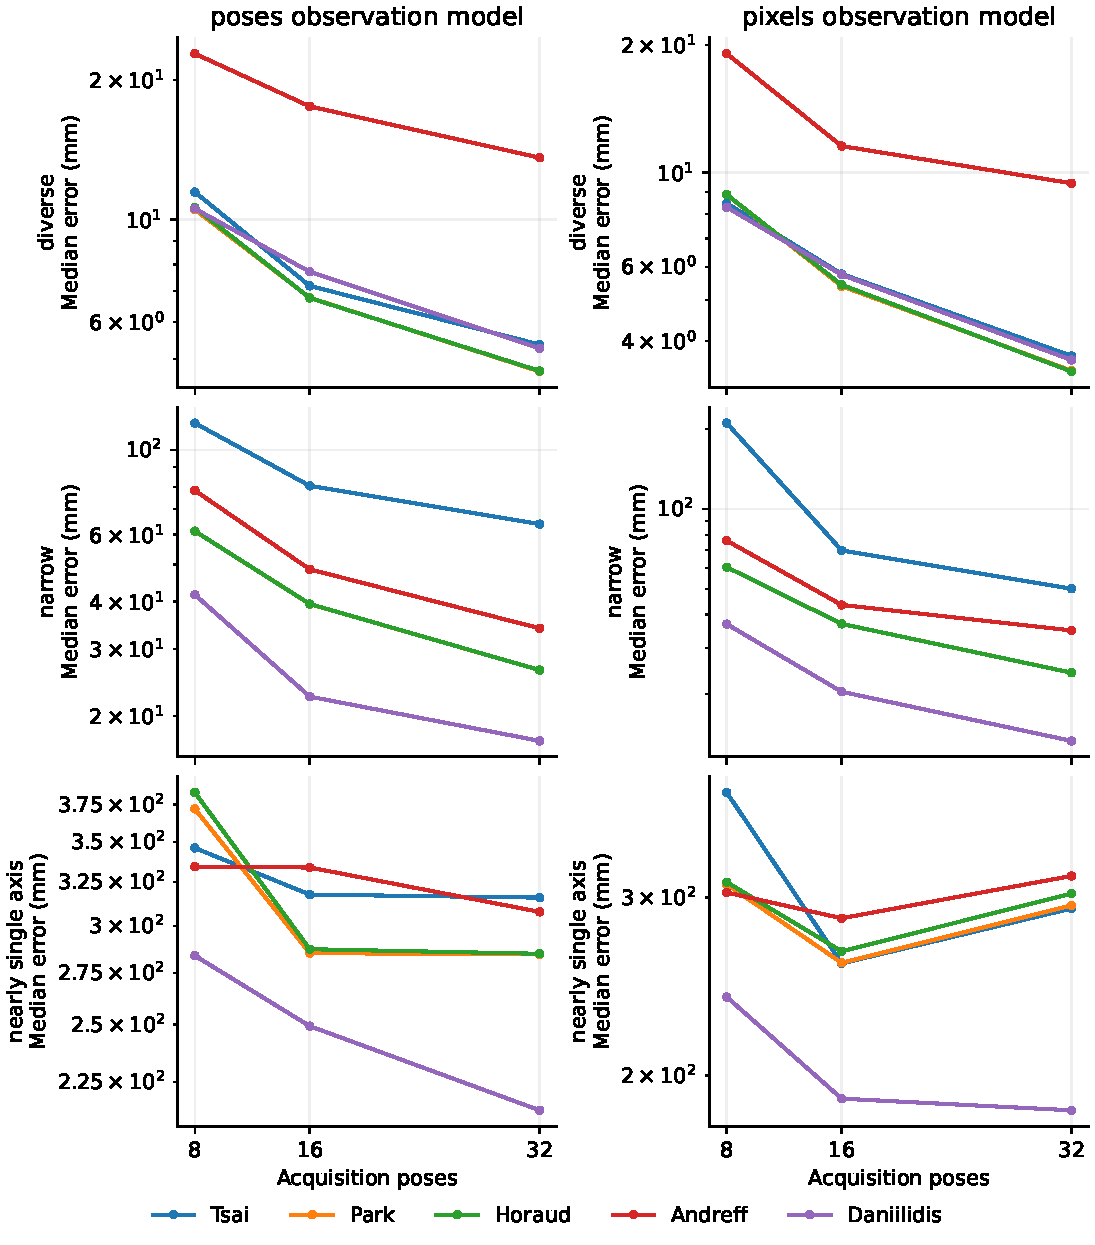
\includegraphics[width=\linewidth]{controlled_sensitivity.pdf}
\caption{Median translation error for the high-noise controlled experiments. All panels use logarithmic vertical axes; columns distinguish the pose and pixel models, and rows distinguish orientation profiles. Pose counts are 8, 16 and 32; each point summarises 100 attempts with errors aggregated over valid estimates.}
\label{fig:controlled}
\end{figure}

Figure~\ref{fig:controlled} shows the effect of pose count and orientation profile without collapsing them into one solver ranking. Diverse orientations produce much smaller errors than the nearly single-axis profile in these runs. In the high-noise, 32-pose diverse conditions, Park and Horaud give median translation errors near 4.70 mm in the pose model and 3.40 mm in the pixel model. Their 32-pose narrow-profile medians remain around 26.4 mm and 24.1 mm respectively. These are measured condition-specific results, rather than a guarantee for other trajectories. \cite{experimentcode}

\begin{table}[!htbp]\centering\footnotesize\setlength{\tabcolsep}{4pt}
\caption{Nearly single-axis profile, 32 poses and high noise. Translation errors remain in mm; all five methods return valid outputs in the pose model, while Park has one rejected output in the pixel model.}\label{tab:axis-tails}
\begin{tabular}{lrrrr}
\toprule
Method & Med. $e_t$, poses & $p_{95}$, poses & Med. $e_t$, pixels & $p_{95}$, pixels \\
\midrule
Tsai & $315.9$ & $620.8$ & $292.7$ & $537.2$ \\
Park & $284.5$ & $595.1$ & $294.7$ & $542$ \\
Horaud & $284.8$ & $601.3$ & $302.8$ & $544.2$ \\
Andreff & $307.7$ & $495.9$ & $315.2$ & $446.4$ \\
Daniilidis & $213.5$ & $6.027\times10^{4}$ & $184.7$ & $5.172\times10^{4}$ \\
\bottomrule
\end{tabular}
\end{table}


The nearly single-axis conditions also show why medians and validity counts are insufficient alone. Daniilidis has median translation errors of about 213.5 mm and 184.7 mm at high noise with 32 poses, but its 95th-percentile errors reach about 60.3 m and 51.7 m in the pose and pixel models. These finite outputs satisfy the wrapper's rigid-transform checks and are retained as large errors. The trajectory-replay median advantage reported next must therefore not be generalised into a universal robustness claim. \cite{experimentcode}

\subsection{Recorded-trajectory simulation}
All 60 replay summary rows were reproduced exactly. Table~\ref{tab:replay-low} gives the 20-pose low-noise condition. Daniilidis has the smallest median translation error, 0.962 mm, while Horaud has the smallest median angle, approximately $0.1051^\circ$, closely followed by Park. Andreff gives a larger median translation error of 1.786 mm. No outputs are rejected in any of the recorded replay conditions. The complete replay summaries are in Appendix~\ref{app:replay}. \cite{experimentcode}

\begin{table}[!htbp]\centering\small
\caption{Trajectory replay: 20 poses, low noise, 100 trials per method.}\label{tab:replay-low}
\begin{tabular}{lrrrr}
\toprule
Method & Med. $e_R$ ($^\circ$) & Med. $e_t$ (mm) & $p_{95}(e_t)$ (mm) & Failed \\
\midrule
Tsai & $0.1205$ & $1.088$ & $2.059$ & 0 \\
Park & $0.1058$ & $1.122$ & $2.156$ & 0 \\
Horaud & $0.1051$ & $1.127$ & $2.16$ & 0 \\
Andreff & $0.1691$ & $1.786$ & $3.485$ & 0 \\
Daniilidis & $0.1363$ & $0.9624$ & $1.993$ & 0 \\
\bottomrule
\end{tabular}
\end{table}


\begin{figure}[!htbp]\centering
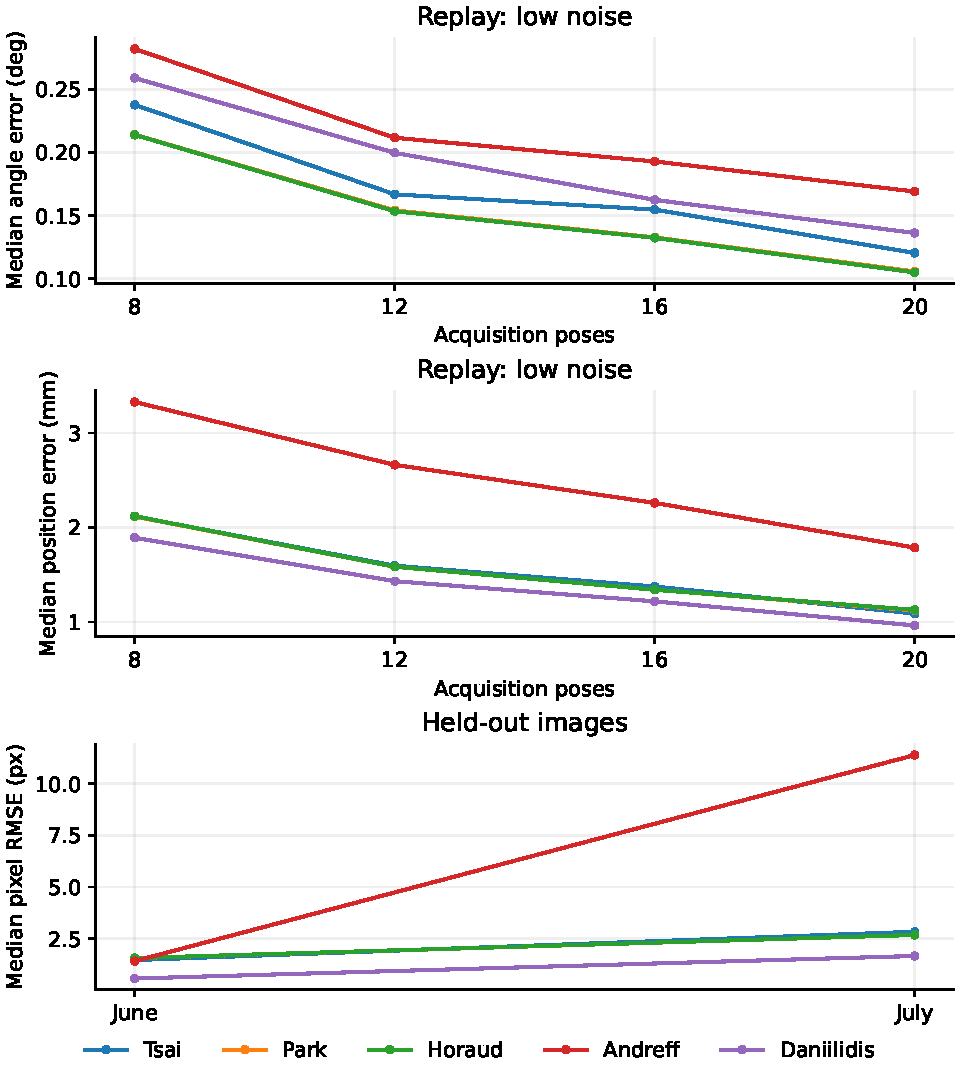
\includegraphics[width=\linewidth]{comparison.pdf}
\caption{Top and middle: low-noise trajectory-replay medians versus acquisition count. Bottom: median held-out pixel RMSE for the June and July series. The image-validation scores and synthetic pose errors have different reference meanings.}
\label{fig:comparison}
\end{figure}

Figure~\ref{fig:comparison} records the pose-count trend on this trajectory. Increasing the number of observations reduces the plotted low-noise median errors. The trajectory, nominal camera, mount and intrinsic model are fixed throughout; these trials do not sample independent camera installations or physical acquisitions. \cite{experimentcode}

\subsection{Held-out laboratory predictions}
The recomputed 15-view June and 18-view July validations reproduce all ten published method/series summary rows, including their medians and 95th percentiles. Daniilidis gives the smallest median pixel RMSE in both series: 0.571 px in June and 1.662 px in July. Park and Horaud have almost identical July pose-space medians. Andreff's July median pixel RMSE is 11.386 px, although its median angular disagreement is comparable to the other methods. This illustrates the value of retaining both image and pose-space scores. \cite{experimentcode}

\begin{table}[!htbp]\centering\footnotesize\setlength{\tabcolsep}{4pt}
\caption{Leave-one-pose-out image prediction. Each method has 15 June and 18 July predictions.}\label{tab:real}
\begin{tabular}{llrrrr}
\toprule
Series & Method & Med. $e_R$ ($^\circ$) & Med. $e_t$ (mm) & Med. RMSE (px) & $p_{95}$ RMSE (px) \\
\midrule
June & Tsai & $0.07789$ & $0.4332$ & $1.465$ & $3.832$ \\
June & Park & $0.07301$ & $0.4221$ & $1.559$ & $4.119$ \\
June & Horaud & $0.0729$ & $0.4223$ & $1.561$ & $4.116$ \\
June & Andreff & $0.07965$ & $0.5821$ & $1.414$ & $3.818$ \\
June & Daniilidis & $0.07448$ & $0.2119$ & $0.5709$ & $2.307$ \\
July & Tsai & $0.1467$ & $0.6534$ & $2.833$ & $5.873$ \\
July & Park & $0.1239$ & $0.5585$ & $2.68$ & $5.516$ \\
July & Horaud & $0.1241$ & $0.5584$ & $2.68$ & $5.535$ \\
July & Andreff & $0.1265$ & $1.829$ & $11.39$ & $20.9$ \\
July & Daniilidis & $0.1342$ & $0.6461$ & $1.662$ & $4.994$ \\
\bottomrule
\end{tabular}
\end{table}


The image score includes camera intrinsics, distortion, target-pose estimation, the hand--eye estimate and the fixed-mount reference. It is not an isolated measurement of one solver's absolute camera-pose error. The two series use different camera records, optics, image sizes and observations; their difference cannot be attributed to the solver alone. Small median differences are not accompanied here by an inferential test based on independent acquisitions. \cite{experimentcode,eauncertainty}

\subsection{Circular target and interpretation of correspondence}\label{sec:circle-results}
For the nine detected circular grids, pose-ID pairing gives a median relative-angle discrepancy of $0.077^\circ$ and a maximum of $0.383^\circ$. The current script's post-detection row-order baseline gives $13.989^\circ$ and $60.897^\circ$. Pairing the 11 raw image entries to robot rows before discarding the two failed detections instead gives a median of $12.997^\circ$ and maximum of $46.441^\circ$. The baseline construction changes the numerical comparison; the low pose-ID discrepancy remains unchanged. \cite{experimentcode}

These results support using the identifiers P40, P42, P48, P49, P51, P52, P56, P57 and P59 for the detected views. They do not validate circle spacing, metric translation, a complete circular-target calibration, or the cause of a historical failure for which the original processing configuration is unavailable. The circular diagnostic is therefore reported separately from the checkerboard validation. \cite{experimentcode}

\subsection{Verification record and reproducibility limits}
The reproduced record comprises 27,000 controlled synthetic attempts, 6,000 trajectory-replay attempts and 165 held-out image predictions. The 270 controlled summary rows, 60 replay rows and ten held-out summary rows matched the published numerical values. An additional exact 32-pose diverse sample recovered the synthetic camera with all five methods; the largest angle error in that check was approximately $3.46\times10^{-12}$ degrees and the largest translation error $2.43\times10^{-11}$ mm. The exact coordinate-loop residual was below $2.28\times10^{-13}$ mm. These are numerical checks for the recorded configurations, not proofs of correctness for every input. \cite{experimentcode}

The repository records source code, pinned numerical dependencies, condition summaries, per-view held-out scores, inferred June corrections and the nominal replay geometry. \code{scripts/build_paper_results.py} rebuilds the printed tables and figures from those recorded outputs; it does not rerun calibration. Trial-level synthetic files are regenerated by the documented commands. Full image processing requires the separately supplied archive. Known limitations include absent robot reachability checks, unmodelled detector failures in synthetic data, unconfirmed physical pixel pitch, the unfinished row-order diagnostic handling and missing per-fold failure recording in real validation. There is no automated regression-test suite or CI workflow for the numerical pipeline in this revision. \cite{experimentcode}

\clearpage
\section{Conclusion}\label{sec:conclusion}
The completed study compares the five OpenCV methods through two controlled observation models, a recorded-trajectory simulation and held-out laboratory image prediction. The theoretical account is restricted to the evaluated solver formulations. The implementation uses consistent eye-to-hand frame directions and separates known-reference simulation errors from real-image prediction consistency. \cite{experimentcode,opencv}

Daniilidis gives the smallest median translation error in the reported 20-pose low-noise replay and the smallest median held-out pixel RMSE in both laboratory series. Park and Horaud give similar behaviour in several controlled and July validation conditions. These findings depend on the tested data and metric: the nearly single-axis experiments expose large finite errors and heavy tails, and narrow rotations can trigger OpenCV's internal Tsai rejection. Reporting distributions and failures is consequently essential to interpreting the comparison. \cite{experimentcode,opencvsource}

The circular-target rotation check supports pose-ID correspondence among the detected views. A complete metric circular-target calibration and an independent laboratory camera-pose reference have not been established. The results support conclusions about the implemented numerical scenarios and prediction consistency of the available recordings; they do not establish absolute physical accuracy or a universally superior method. \cite{experimentcode,eauncertainty}

\clearpage
\appendix
\clearpage
\section{Implementation Inventory}\label{app:functions}
The inventory describes the source revision used for the recorded runs. Public helper functions and command-line entry points are included so that the computational sequence can be traced without adding general matrix-algebra exposition. \cite{experimentcode}
\small
\begin{longtable}{p{0.34\linewidth}p{0.59\linewidth}}
\caption{Functions in \code{benchmark.py}.}\label{tab:benchmark-functions}\\
\toprule Function & Role\\\midrule\endfirsthead
\toprule Function & Role\\\midrule\endhead
\bottomrule\endfoot
\code{transform} & Converts one rotation vector and translation to a homogeneous pose.\\
\code{inverse} & Computes the rigid inverse using $R^\top$ and $-R^\top t$.\\
\code{noisy_pose} & Applies a valid small left rotation and an independent frame-origin position perturbation.\\
\code{observed_target} & Projects the generic target, checks ideal visibility, perturbs image coordinates and estimates the target pose with iterative PnP.\\
\code{observations} & Creates a paired trial and returns inverse robot poses and camera-side target poses.\\
\code{solve_handeye} & Calls the selected OpenCV method and checks finite values, rotation validity and the experiment-specific identity fallback.\\
\code{pose_error} & Returns relative rotation angle in degrees and Euclidean translation disagreement in mm.\\
\code{estimate} & Compares a method estimate with the generic synthetic camera truth.\\
\code{write_csv} & Writes a list of dictionaries with a header.\\
\code{run} & Sweeps 27 conditions, repeats paired trials and saves raw and summary tables.\\
Command-line entry & Reads seed, trials, model and output folder; checks positive trial count and nonnegative seed.\\
\end{longtable}
\begin{longtable}{p{0.34\linewidth}p{0.59\linewidth}}
\caption{Functions in \code{laboratory.py} and \code{circle_diagnostic.py}.}\label{tab:laboratory-functions}\\
\toprule Function & Role\\\midrule\endfirsthead
\toprule Function & Role\\\midrule\endhead
\bottomrule\endfoot
\code{june_poses} & Parses the June ODS XML, returns 15 poses and logs the eight inferred corrections.\\
\code{read_series} & Pairs images by pose identifier, detects/refines checkerboard corners and converts robot Euler angles.\\
\code{camera_fit} & Fits camera intrinsics, distortion and per-image target poses.\\
\code{target_pose} & Fits one target pose with PnP using fixed intrinsics and distortion.\\
\code{project} & Projects the 88 laboratory target points; adds no noise or visibility rejection itself.\\
\code{mount_pose} & Averages training-implied target-to-TCP mounts and projects the rotation mean to a proper rotation.\\
\code{validate} & Refits on training views, predicts each held-out view and records pose-space and image-space disagreement.\\
Laboratory \code{run} & Audits the series, defines nominal geometry, runs both real validations and sweeps the trajectory simulation.\\
\code{rotation_angle} & Computes the principal angle between two rotation matrices.\\
\code{compare} & Detects circular grids and compares relative-angle discrepancies for the two correspondence baselines.\\
Command-line entries & Read the archive path and, for laboratory processing, trial count, seed and output folder.\\
\end{longtable}
\normalsize

\clearpage
\section{Complete Controlled Synthetic Summaries}\label{app:controlled}
Each row represents 100 attempts. Angular errors are in degrees and translation errors in mm. Medians and 95th percentiles include valid estimates only; failed outputs are counted separately. The tables reproduce \code{results/poses/summary.csv} and \code{results/pixels/summary.csv}, rounded to four significant digits for printing. \cite{experimentcode}
\begingroup\small\setlength{\tabcolsep}{4pt}
\begin{longtable}{rllrrrrr}
\caption{Controlled poses model, diverse profile; 100 trials per row.}\label{tab:poses-diverse}\\
\toprule
$N$ & Noise & Method & Failed & Med. $e_R$ & $p_{95}(e_R)$ & Med. $e_t$ & $p_{95}(e_t)$ \\
\midrule
\endfirsthead
\multicolumn{8}{l}{\small\tablename~\thetable\ (continued)}\\
\toprule
$N$ & Noise & Method & Failed & Med. $e_R$ & $p_{95}(e_R)$ & Med. $e_t$ & $p_{95}(e_t)$ \\
\midrule
\endhead
\midrule
\multicolumn{8}{r}{\small Continued on next page}\\
\endfoot
\bottomrule
\endlastfoot
8 & exact & Tsai & 0 & $1.351\times10^{-13}$ & $2.554\times10^{-13}$ & $1.095\times10^{-12}$ & $2.276\times10^{-12}$ \\
8 & exact & Park & 0 & $1.059\times10^{-14}$ & $4.266\times10^{-14}$ & $6.265\times10^{-13}$ & $2.076\times10^{-12}$ \\
8 & exact & Horaud & 0 & $1.368\times10^{-14}$ & $3.111\times10^{-14}$ & $6.592\times10^{-13}$ & $1.899\times10^{-12}$ \\
8 & exact & Andreff & 0 & $5.44\times10^{-12}$ & $1.376\times10^{-11}$ & $2.465\times10^{-11}$ & $7.819\times10^{-11}$ \\
8 & exact & Daniilidis & 0 & $9.172\times10^{-14}$ & $1.158\times10^{-12}$ & $7.509\times10^{-13}$ & $3.597\times10^{-12}$ \\
8 & low & Tsai & 0 & $0.2043$ & $0.4456$ & $2.164$ & $4.406$ \\
8 & low & Park & 0 & $0.1692$ & $0.3196$ & $2.152$ & $4.316$ \\
8 & low & Horaud & 0 & $0.1709$ & $0.3191$ & $2.162$ & $4.32$ \\
8 & low & Andreff & 0 & $0.231$ & $0.5135$ & $4.003$ & $10.89$ \\
8 & low & Daniilidis & 0 & $0.266$ & $0.6146$ & $2.271$ & $4.533$ \\
8 & high & Tsai & 0 & $1.12$ & $2.291$ & $11.47$ & $21.69$ \\
8 & high & Park & 0 & $0.852$ & $1.611$ & $10.51$ & $20.69$ \\
8 & high & Horaud & 0 & $0.8579$ & $1.609$ & $10.61$ & $20.87$ \\
8 & high & Andreff & 0 & $1.074$ & $2.495$ & $22.82$ & $64.69$ \\
8 & high & Daniilidis & 0 & $1.228$ & $3.061$ & $10.56$ & $22.52$ \\
16 & exact & Tsai & 0 & $1.352\times10^{-13}$ & $2.551\times10^{-13}$ & $1.275\times10^{-12}$ & $2.338\times10^{-12}$ \\
16 & exact & Park & 0 & $6.884\times10^{-15}$ & $1.903\times10^{-14}$ & $7.045\times10^{-13}$ & $1.461\times10^{-12}$ \\
16 & exact & Horaud & 0 & $1.669\times10^{-14}$ & $3.867\times10^{-14}$ & $8.183\times10^{-13}$ & $1.872\times10^{-12}$ \\
16 & exact & Andreff & 0 & $4.688\times10^{-12}$ & $2.739\times10^{-11}$ & $3.097\times10^{-11}$ & $8.798\times10^{-11}$ \\
16 & exact & Daniilidis & 0 & $1.355\times10^{-13}$ & $8.263\times10^{-13}$ & $9.672\times10^{-13}$ & $5.665\times10^{-12}$ \\
16 & low & Tsai & 0 & $0.1367$ & $0.2732$ & $1.395$ & $2.71$ \\
16 & low & Park & 0 & $0.113$ & $0.2156$ & $1.428$ & $2.503$ \\
16 & low & Horaud & 0 & $0.1091$ & $0.2164$ & $1.42$ & $2.535$ \\
16 & low & Andreff & 0 & $0.1309$ & $0.24$ & $2.803$ & $6.895$ \\
16 & low & Daniilidis & 0 & $0.1542$ & $0.3353$ & $1.516$ & $2.67$ \\
16 & high & Tsai & 0 & $0.8853$ & $1.605$ & $7.19$ & $15.4$ \\
16 & high & Park & 0 & $0.5661$ & $1.08$ & $6.78$ & $12.14$ \\
16 & high & Horaud & 0 & $0.5454$ & $1.084$ & $6.772$ & $12.29$ \\
16 & high & Andreff & 0 & $0.6359$ & $1.2$ & $17.55$ & $42.9$ \\
16 & high & Daniilidis & 0 & $0.7313$ & $2.274$ & $7.713$ & $14.36$ \\
32 & exact & Tsai & 0 & $1.371\times10^{-13}$ & $2.55\times10^{-13}$ & $1.542\times10^{-12}$ & $2.766\times10^{-12}$ \\
32 & exact & Park & 0 & $8.529\times10^{-15}$ & $2.662\times10^{-14}$ & $1.039\times10^{-12}$ & $2.281\times10^{-12}$ \\
32 & exact & Horaud & 0 & $2.364\times10^{-14}$ & $4.629\times10^{-14}$ & $1.119\times10^{-12}$ & $2.538\times10^{-12}$ \\
32 & exact & Andreff & 0 & $5.665\times10^{-12}$ & $2.786\times10^{-11}$ & $2.426\times10^{-11}$ & $8.563\times10^{-11}$ \\
32 & exact & Daniilidis & 0 & $1.359\times10^{-13}$ & $6.268\times10^{-13}$ & $8.836\times10^{-13}$ & $5.257\times10^{-12}$ \\
32 & low & Tsai & 0 & $0.09475$ & $0.1671$ & $0.9968$ & $1.758$ \\
32 & low & Park & 0 & $0.07212$ & $0.1304$ & $0.9959$ & $1.788$ \\
32 & low & Horaud & 0 & $0.07248$ & $0.1313$ & $1.005$ & $1.766$ \\
32 & low & Andreff & 0 & $0.08438$ & $0.145$ & $1.858$ & $4.947$ \\
32 & low & Daniilidis & 0 & $0.1062$ & $0.1967$ & $1.036$ & $2.037$ \\
32 & high & Tsai & 0 & $0.7187$ & $1.142$ & $5.371$ & $10.13$ \\
32 & high & Park & 0 & $0.3608$ & $0.652$ & $4.698$ & $8.919$ \\
32 & high & Horaud & 0 & $0.3624$ & $0.6493$ & $4.71$ & $8.806$ \\
32 & high & Andreff & 0 & $0.4152$ & $0.7185$ & $13.6$ & $31.14$ \\
32 & high & Daniilidis & 0 & $0.495$ & $0.9762$ & $5.271$ & $10.43$ \\
\end{longtable}
\endgroup

\begingroup\footnotesize\setlength{\tabcolsep}{2pt}
\begin{longtable}{rllrrrrr}
\caption{Controlled poses model, narrow profile; 100 trials per row.}\label{tab:poses-narrow}\\
\toprule
$N$ & Noise & Method & Failed & Med. $e_R$ & $p_{95}(e_R)$ & Med. $e_t$ & $p_{95}(e_t)$ \\
\midrule
\endfirsthead
\multicolumn{8}{l}{\small\tablename~\thetable\ (continued)}\\
\toprule
$N$ & Noise & Method & Failed & Med. $e_R$ & $p_{95}(e_R)$ & Med. $e_t$ & $p_{95}(e_t)$ \\
\midrule
\endhead
\midrule
\multicolumn{8}{r}{\small Continued on next page}\\
\endfoot
\bottomrule
\endlastfoot
8 & exact & Tsai & 81 & $1.68\times10^{-13}$ & $2.845\times10^{-13}$ & $2.313\times10^{-12}$ & $8.806\times10^{-12}$ \\
8 & exact & Park & 0 & $1.385\times10^{-14}$ & $5.615\times10^{-14}$ & $9.596\times10^{-13}$ & $4.111\times10^{-12}$ \\
8 & exact & Horaud & 0 & $1.935\times10^{-14}$ & $3.858\times10^{-14}$ & $8.286\times10^{-13}$ & $2.463\times10^{-12}$ \\
8 & exact & Andreff & 0 & $4.534\times10^{-12}$ & $1.072\times10^{-11}$ & $4.88\times10^{-11}$ & $1.237\times10^{-10}$ \\
8 & exact & Daniilidis & 0 & $9.618\times10^{-14}$ & $7.528\times10^{-13}$ & $1.153\times10^{-12}$ & $9.35\times10^{-12}$ \\
8 & low & Tsai & 82 & $1.501$ & $11.36$ & $30.22$ & $288.6$ \\
8 & low & Park & 0 & $0.875$ & $1.847$ & $12.83$ & $23.47$ \\
8 & low & Horaud & 0 & $0.875$ & $1.847$ & $12.83$ & $23.47$ \\
8 & low & Andreff & 0 & $0.9394$ & $1.848$ & $15.74$ & $39.18$ \\
8 & low & Daniilidis & 0 & $0.678$ & $1.548$ & $9.425$ & $18.81$ \\
8 & high & Tsai & 86 & $8.038$ & $103.2$ & $117.6$ & $2291$ \\
8 & high & Park & 0 & $4.496$ & $9.329$ & $61.18$ & $113.8$ \\
8 & high & Horaud & 0 & $4.497$ & $9.329$ & $61.19$ & $113.8$ \\
8 & high & Andreff & 0 & $4.198$ & $9.016$ & $78.25$ & $184.8$ \\
8 & high & Daniilidis & 0 & $3.088$ & $6.275$ & $41.66$ & $85.41$ \\
16 & exact & Tsai & 42 & $1.448\times10^{-13}$ & $2.617\times10^{-13}$ & $1.584\times10^{-12}$ & $4.408\times10^{-12}$ \\
16 & exact & Park & 0 & $8.805\times10^{-15}$ & $2.291\times10^{-14}$ & $7.999\times10^{-13}$ & $1.666\times10^{-12}$ \\
16 & exact & Horaud & 0 & $1.716\times10^{-14}$ & $3.866\times10^{-14}$ & $9.688\times10^{-13}$ & $1.993\times10^{-12}$ \\
16 & exact & Andreff & 0 & $4.094\times10^{-12}$ & $1.183\times10^{-11}$ & $3.256\times10^{-11}$ & $1.085\times10^{-10}$ \\
16 & exact & Daniilidis & 0 & $1.145\times10^{-13}$ & $1.007\times10^{-12}$ & $1.591\times10^{-12}$ & $8.317\times10^{-12}$ \\
16 & low & Tsai & 42 & $1.137$ & $3.544$ & $14.32$ & $37.98$ \\
16 & low & Park & 0 & $0.5869$ & $1.115$ & $7.74$ & $14.59$ \\
16 & low & Horaud & 0 & $0.5874$ & $1.115$ & $7.737$ & $14.59$ \\
16 & low & Andreff & 0 & $0.5004$ & $0.8937$ & $9.298$ & $16.32$ \\
16 & low & Daniilidis & 0 & $0.3765$ & $0.6744$ & $5.065$ & $9.574$ \\
16 & high & Tsai & 44 & $7.783$ & $46.78$ & $80.46$ & $494.9$ \\
16 & high & Park & 0 & $2.942$ & $5.814$ & $39.38$ & $70.23$ \\
16 & high & Horaud & 0 & $2.946$ & $5.813$ & $39.4$ & $70.23$ \\
16 & high & Andreff & 0 & $2.427$ & $4.345$ & $48.57$ & $105.9$ \\
16 & high & Daniilidis & 0 & $1.642$ & $3.143$ & $22.5$ & $44.58$ \\
32 & exact & Tsai & 5 & $1.358\times10^{-13}$ & $2.588\times10^{-13}$ & $1.311\times10^{-12}$ & $3.079\times10^{-12}$ \\
32 & exact & Park & 0 & $7.911\times10^{-15}$ & $1.986\times10^{-14}$ & $1.112\times10^{-12}$ & $2.631\times10^{-12}$ \\
32 & exact & Horaud & 0 & $2.377\times10^{-14}$ & $4.964\times10^{-14}$ & $1.275\times10^{-12}$ & $2.905\times10^{-12}$ \\
32 & exact & Andreff & 0 & $4.829\times10^{-12}$ & $2.269\times10^{-11}$ & $3.313\times10^{-11}$ & $9.507\times10^{-11}$ \\
32 & exact & Daniilidis & 0 & $1.071\times10^{-13}$ & $2.178\times10^{-12}$ & $1.295\times10^{-12}$ & $1.177\times10^{-11}$ \\
32 & low & Tsai & 6 & $0.7974$ & $1.677$ & $8.269$ & $19.89$ \\
32 & low & Park & 0 & $0.4218$ & $0.6763$ & $5.491$ & $10.29$ \\
32 & low & Horaud & 0 & $0.4218$ & $0.6765$ & $5.491$ & $10.3$ \\
32 & low & Andreff & 0 & $0.3029$ & $0.5586$ & $5.774$ & $11.32$ \\
32 & low & Daniilidis & 0 & $0.2302$ & $0.4156$ & $3.679$ & $7.799$ \\
32 & high & Tsai & 7 & $7.091$ & $34.94$ & $63.84$ & $339.4$ \\
32 & high & Park & 0 & $2.162$ & $3.322$ & $26.42$ & $53.97$ \\
32 & high & Horaud & 0 & $2.16$ & $3.323$ & $26.42$ & $53.96$ \\
32 & high & Andreff & 0 & $1.44$ & $2.783$ & $34.01$ & $71.8$ \\
32 & high & Daniilidis & 0 & $1.056$ & $2.181$ & $17.22$ & $38.42$ \\
\end{longtable}
\endgroup

\begingroup\footnotesize\setlength{\tabcolsep}{2pt}
\begin{longtable}{rllrrrrr}
\caption{Controlled poses model, nearly single axis profile; 100 trials per row.}\label{tab:poses-nearly-single-axis}\\
\toprule
$N$ & Noise & Method & Failed & Med. $e_R$ & $p_{95}(e_R)$ & Med. $e_t$ & $p_{95}(e_t)$ \\
\midrule
\endfirsthead
\multicolumn{8}{l}{\small\tablename~\thetable\ (continued)}\\
\toprule
$N$ & Noise & Method & Failed & Med. $e_R$ & $p_{95}(e_R)$ & Med. $e_t$ & $p_{95}(e_t)$ \\
\midrule
\endhead
\midrule
\multicolumn{8}{r}{\small Continued on next page}\\
\endfoot
\bottomrule
\endlastfoot
8 & exact & Tsai & 0 & $2.124\times10^{-13}$ & $4.471\times10^{-13}$ & $3.957\times10^{-12}$ & $1.404\times10^{-11}$ \\
8 & exact & Park & 0 & $5.254\times10^{-11}$ & $1.287\times10^{-9}$ & $1.159\times10^{-8}$ & $3.244\times10^{-7}$ \\
8 & exact & Horaud & 0 & $4.505\times10^{-14}$ & $2.925\times10^{-13}$ & $2.83\times10^{-12}$ & $1.686\times10^{-11}$ \\
8 & exact & Andreff & 0 & $4.311\times10^{-12}$ & $1.134\times10^{-11}$ & $2.157\times10^{-11}$ & $1.195\times10^{-10}$ \\
8 & exact & Daniilidis & 0 & $8.535\times10^{-14}$ & $4.038\times10^{-13}$ & $4.673\times10^{-12}$ & $1.135\times10^{-11}$ \\
8 & low & Tsai & 0 & $4.782$ & $14.15$ & $104.1$ & $692$ \\
8 & low & Park & 0 & $3.209$ & $11.14$ & $82.44$ & $401.3$ \\
8 & low & Horaud & 0 & $3.204$ & $11.15$ & $82.39$ & $399.8$ \\
8 & low & Andreff & 0 & $0.9314$ & $2.09$ & $56.24$ & $168.7$ \\
8 & low & Daniilidis & 0 & $0.5776$ & $1.338$ & $40.43$ & $128.4$ \\
8 & high & Tsai & 0 & $18.7$ & $50.85$ & $346.1$ & $1274$ \\
8 & high & Park & 15 & $15.98$ & $71.35$ & $372$ & $1272$ \\
8 & high & Horaud & 0 & $18.07$ & $81.34$ & $383.4$ & $1522$ \\
8 & high & Andreff & 0 & $3.969$ & $9.156$ & $334.5$ & $777.9$ \\
8 & high & Daniilidis & 0 & $2.742$ & $153.6$ & $283.8$ & $1.247\times10^{4}$ \\
16 & exact & Tsai & 0 & $1.905\times10^{-13}$ & $4.178\times10^{-13}$ & $2.274\times10^{-12}$ & $1.055\times10^{-11}$ \\
16 & exact & Park & 0 & $1.826\times10^{-11}$ & $2.226\times10^{-10}$ & $2.403\times10^{-9}$ & $3.315\times10^{-8}$ \\
16 & exact & Horaud & 0 & $7.994\times10^{-14}$ & $2.817\times10^{-13}$ & $1.904\times10^{-12}$ & $7.901\times10^{-12}$ \\
16 & exact & Andreff & 0 & $3.897\times10^{-12}$ & $1.502\times10^{-11}$ & $1.231\times10^{-11}$ & $7.893\times10^{-11}$ \\
16 & exact & Daniilidis & 0 & $7.129\times10^{-14}$ & $4.642\times10^{-13}$ & $3.923\times10^{-12}$ & $7.555\times10^{-12}$ \\
16 & low & Tsai & 0 & $2.916$ & $9.092$ & $49.62$ & $248.6$ \\
16 & low & Park & 0 & $2.395$ & $6.369$ & $39.97$ & $216.7$ \\
16 & low & Horaud & 0 & $2.398$ & $6.343$ & $40.16$ & $216.1$ \\
16 & low & Andreff & 0 & $0.5531$ & $0.9868$ & $36.94$ & $101.8$ \\
16 & low & Daniilidis & 0 & $0.3152$ & $0.6449$ & $26.97$ & $69.05$ \\
16 & high & Tsai & 0 & $11.76$ & $30.54$ & $317.7$ & $692.8$ \\
16 & high & Park & 4 & $16.31$ & $45.7$ & $285.2$ & $754$ \\
16 & high & Horaud & 0 & $16.24$ & $45.21$ & $287.2$ & $771.1$ \\
16 & high & Andreff & 0 & $2.254$ & $4.131$ & $333.9$ & $537.8$ \\
16 & high & Daniilidis & 0 & $1.608$ & $163.1$ & $249.3$ & $3.07\times10^{4}$ \\
32 & exact & Tsai & 0 & $1.688\times10^{-13}$ & $7.691\times10^{-13}$ & $2.111\times10^{-12}$ & $6.557\times10^{-12}$ \\
32 & exact & Park & 0 & $1.271\times10^{-11}$ & $1.27\times10^{-10}$ & $1.341\times10^{-9}$ & $1.516\times10^{-8}$ \\
32 & exact & Horaud & 0 & $1.722\times10^{-13}$ & $5.492\times10^{-13}$ & $2.055\times10^{-12}$ & $8.345\times10^{-12}$ \\
32 & exact & Andreff & 0 & $4.035\times10^{-12}$ & $1.097\times10^{-11}$ & $1.013\times10^{-11}$ & $4.699\times10^{-11}$ \\
32 & exact & Daniilidis & 0 & $9.779\times10^{-14}$ & $8.638\times10^{-13}$ & $3.669\times10^{-12}$ & $6.669\times10^{-12}$ \\
32 & low & Tsai & 0 & $1.48$ & $5.283$ & $26.72$ & $111.4$ \\
32 & low & Park & 0 & $1.787$ & $3.99$ & $30.76$ & $90.79$ \\
32 & low & Horaud & 0 & $1.784$ & $3.999$ & $30.85$ & $90.74$ \\
32 & low & Andreff & 0 & $0.3296$ & $0.5751$ & $23.64$ & $67.47$ \\
32 & low & Daniilidis & 0 & $0.2065$ & $0.3914$ & $22.31$ & $50.04$ \\
32 & high & Tsai & 0 & $6.828$ & $21.38$ & $315.9$ & $620.8$ \\
32 & high & Park & 0 & $10.11$ & $25.9$ & $284.5$ & $595.1$ \\
32 & high & Horaud & 0 & $10.07$ & $25.9$ & $284.8$ & $601.3$ \\
32 & high & Andreff & 0 & $1.488$ & $2.457$ & $307.7$ & $495.9$ \\
32 & high & Daniilidis & 0 & $1.08$ & $172.8$ & $213.5$ & $6.027\times10^{4}$ \\
\end{longtable}
\endgroup

\begingroup\footnotesize\setlength{\tabcolsep}{2pt}
\begin{longtable}{rllrrrrr}
\caption{Controlled pixels model, diverse profile; 100 trials per row.}\label{tab:pixels-diverse}\\
\toprule
$N$ & Noise & Method & Failed & Med. $e_R$ & $p_{95}(e_R)$ & Med. $e_t$ & $p_{95}(e_t)$ \\
\midrule
\endfirsthead
\multicolumn{8}{l}{\small\tablename~\thetable\ (continued)}\\
\toprule
$N$ & Noise & Method & Failed & Med. $e_R$ & $p_{95}(e_R)$ & Med. $e_t$ & $p_{95}(e_t)$ \\
\midrule
\endhead
\midrule
\multicolumn{8}{r}{\small Continued on next page}\\
\endfoot
\bottomrule
\endlastfoot
8 & exact & Tsai & 0 & $2.903\times10^{-8}$ & $9.706\times10^{-8}$ & $6.407\times10^{-7}$ & $1.67\times10^{-6}$ \\
8 & exact & Park & 0 & $2.942\times10^{-8}$ & $8.504\times10^{-8}$ & $6.677\times10^{-7}$ & $1.814\times10^{-6}$ \\
8 & exact & Horaud & 0 & $2.969\times10^{-8}$ & $8.393\times10^{-8}$ & $6.692\times10^{-7}$ & $1.819\times10^{-6}$ \\
8 & exact & Andreff & 0 & $5.083\times10^{-8}$ & $1.413\times10^{-7}$ & $1.268\times10^{-6}$ & $4.768\times10^{-6}$ \\
8 & exact & Daniilidis & 0 & $3.207\times10^{-8}$ & $1.032\times10^{-7}$ & $4.822\times10^{-7}$ & $1.186\times10^{-6}$ \\
8 & low & Tsai & 0 & $0.1587$ & $0.2873$ & $1.723$ & $3.428$ \\
8 & low & Park & 0 & $0.1367$ & $0.2714$ & $1.785$ & $3.545$ \\
8 & low & Horaud & 0 & $0.1382$ & $0.2745$ & $1.78$ & $3.569$ \\
8 & low & Andreff & 0 & $0.1646$ & $0.4526$ & $3.81$ & $10.58$ \\
8 & low & Daniilidis & 0 & $0.1971$ & $0.4496$ & $1.818$ & $3.697$ \\
8 & high & Tsai & 0 & $0.8539$ & $1.691$ & $8.468$ & $17.64$ \\
8 & high & Park & 0 & $0.662$ & $1.276$ & $8.878$ & $16.98$ \\
8 & high & Horaud & 0 & $0.6655$ & $1.26$ & $8.882$ & $17.02$ \\
8 & high & Andreff & 0 & $0.7545$ & $2.125$ & $19.1$ & $50.68$ \\
8 & high & Daniilidis & 0 & $0.8933$ & $2.172$ & $8.29$ & $17.68$ \\
16 & exact & Tsai & 0 & $2.206\times10^{-8}$ & $4.795\times10^{-8}$ & $3.879\times10^{-7}$ & $8.49\times10^{-7}$ \\
16 & exact & Park & 0 & $1.929\times10^{-8}$ & $4.373\times10^{-8}$ & $4.348\times10^{-7}$ & $8.614\times10^{-7}$ \\
16 & exact & Horaud & 0 & $1.932\times10^{-8}$ & $4.406\times10^{-8}$ & $4.352\times10^{-7}$ & $8.579\times10^{-7}$ \\
16 & exact & Andreff & 0 & $2.828\times10^{-8}$ & $6.174\times10^{-8}$ & $9.145\times10^{-7}$ & $2.346\times10^{-6}$ \\
16 & exact & Daniilidis & 0 & $2.093\times10^{-8}$ & $4.89\times10^{-8}$ & $2.764\times10^{-7}$ & $7.032\times10^{-7}$ \\
16 & low & Tsai & 0 & $0.1038$ & $0.1863$ & $1.15$ & $1.995$ \\
16 & low & Park & 0 & $0.08096$ & $0.1549$ & $1.119$ & $1.975$ \\
16 & low & Horaud & 0 & $0.08114$ & $0.1547$ & $1.131$ & $1.971$ \\
16 & low & Andreff & 0 & $0.0911$ & $0.1961$ & $1.973$ & $5.951$ \\
16 & low & Daniilidis & 0 & $0.1189$ & $0.2277$ & $1.212$ & $2.21$ \\
16 & high & Tsai & 0 & $0.5909$ & $1.083$ & $5.77$ & $10.45$ \\
16 & high & Park & 0 & $0.402$ & $0.7783$ & $5.398$ & $9.672$ \\
16 & high & Horaud & 0 & $0.4036$ & $0.7778$ & $5.437$ & $9.664$ \\
16 & high & Andreff & 0 & $0.4389$ & $0.939$ & $11.56$ & $27.04$ \\
16 & high & Daniilidis & 0 & $0.5659$ & $0.9937$ & $5.743$ & $10.57$ \\
32 & exact & Tsai & 0 & $1.593\times10^{-8}$ & $3.212\times10^{-8}$ & $2.532\times10^{-7}$ & $5.568\times10^{-7}$ \\
32 & exact & Park & 0 & $1.39\times10^{-8}$ & $3.115\times10^{-8}$ & $2.793\times10^{-7}$ & $6.011\times10^{-7}$ \\
32 & exact & Horaud & 0 & $1.392\times10^{-8}$ & $3.163\times10^{-8}$ & $2.778\times10^{-7}$ & $6.024\times10^{-7}$ \\
32 & exact & Andreff & 0 & $1.868\times10^{-8}$ & $3.664\times10^{-8}$ & $5.141\times10^{-7}$ & $1.44\times10^{-6}$ \\
32 & exact & Daniilidis & 0 & $1.455\times10^{-8}$ & $3.73\times10^{-8}$ & $2.275\times10^{-7}$ & $4.786\times10^{-7}$ \\
32 & low & Tsai & 0 & $0.0666$ & $0.1101$ & $0.7115$ & $1.351$ \\
32 & low & Park & 0 & $0.0512$ & $0.0913$ & $0.72$ & $1.339$ \\
32 & low & Horaud & 0 & $0.05191$ & $0.09136$ & $0.7328$ & $1.343$ \\
32 & low & Andreff & 0 & $0.05896$ & $0.1073$ & $1.541$ & $3.68$ \\
32 & low & Daniilidis & 0 & $0.07346$ & $0.1468$ & $0.794$ & $1.434$ \\
32 & high & Tsai & 0 & $0.4459$ & $0.7$ & $3.695$ & $6.914$ \\
32 & high & Park & 0 & $0.2522$ & $0.4708$ & $3.41$ & $6.028$ \\
32 & high & Horaud & 0 & $0.2573$ & $0.4712$ & $3.396$ & $6.034$ \\
32 & high & Andreff & 0 & $0.2904$ & $0.5293$ & $9.445$ & $20.16$ \\
32 & high & Daniilidis & 0 & $0.346$ & $0.6563$ & $3.614$ & $7.194$ \\
\end{longtable}
\endgroup

\begingroup\small\setlength{\tabcolsep}{4pt}
\begin{longtable}{rllrrrrr}
\caption{Controlled pixels model, narrow profile; 100 trials per row.}\label{tab:pixels-narrow}\\
\toprule
$N$ & Noise & Method & Failed & Med. $e_R$ & $p_{95}(e_R)$ & Med. $e_t$ & $p_{95}(e_t)$ \\
\midrule
\endfirsthead
\multicolumn{8}{l}{\small\tablename~\thetable\ (continued)}\\
\toprule
$N$ & Noise & Method & Failed & Med. $e_R$ & $p_{95}(e_R)$ & Med. $e_t$ & $p_{95}(e_t)$ \\
\midrule
\endhead
\midrule
\multicolumn{8}{r}{\small Continued on next page}\\
\endfoot
\bottomrule
\endlastfoot
8 & exact & Tsai & 81 & $2.426\times10^{-7}$ & $1.085\times10^{-6}$ & $3.687\times10^{-6}$ & $1.63\times10^{-5}$ \\
8 & exact & Park & 0 & $1.66\times10^{-7}$ & $3.893\times10^{-7}$ & $3.272\times10^{-6}$ & $8.004\times10^{-6}$ \\
8 & exact & Horaud & 0 & $1.661\times10^{-7}$ & $3.893\times10^{-7}$ & $3.272\times10^{-6}$ & $8.005\times10^{-6}$ \\
8 & exact & Andreff & 0 & $1.911\times10^{-7}$ & $4.844\times10^{-7}$ & $3.277\times10^{-6}$ & $8.757\times10^{-6}$ \\
8 & exact & Daniilidis & 0 & $6.303\times10^{-8}$ & $1.59\times10^{-7}$ & $1.079\times10^{-6}$ & $3.762\times10^{-6}$ \\
8 & low & Tsai & 82 & $2.743$ & $6.065$ & $23.43$ & $124.8$ \\
8 & low & Park & 0 & $0.9385$ & $1.99$ & $13.47$ & $27.77$ \\
8 & low & Horaud & 0 & $0.9388$ & $1.99$ & $13.47$ & $27.77$ \\
8 & low & Andreff & 0 & $0.9442$ & $1.913$ & $17.51$ & $43.04$ \\
8 & low & Daniilidis & 0 & $0.4726$ & $1.122$ & $8.187$ & $18.32$ \\
8 & high & Tsai & 86 & $12.15$ & $88.87$ & $210.9$ & $1399$ \\
8 & high & Park & 0 & $4.457$ & $9.002$ & $60.36$ & $126.6$ \\
8 & high & Horaud & 0 & $4.456$ & $9.006$ & $60.35$ & $126.7$ \\
8 & high & Andreff & 0 & $4.263$ & $7.742$ & $75.99$ & $192.5$ \\
8 & high & Daniilidis & 0 & $2.403$ & $5.178$ & $36.81$ & $83.94$ \\
16 & exact & Tsai & 42 & $1.673\times10^{-7}$ & $4.832\times10^{-7}$ & $2.278\times10^{-6}$ & $6.955\times10^{-6}$ \\
16 & exact & Park & 0 & $1.172\times10^{-7}$ & $2.304\times10^{-7}$ & $2.07\times10^{-6}$ & $4.054\times10^{-6}$ \\
16 & exact & Horaud & 0 & $1.171\times10^{-7}$ & $2.305\times10^{-7}$ & $2.07\times10^{-6}$ & $4.054\times10^{-6}$ \\
16 & exact & Andreff & 0 & $1.01\times10^{-7}$ & $2.259\times10^{-7}$ & $2.062\times10^{-6}$ & $4.334\times10^{-6}$ \\
16 & exact & Daniilidis & 0 & $3.873\times10^{-8}$ & $9.489\times10^{-8}$ & $6.936\times10^{-7}$ & $1.556\times10^{-6}$ \\
16 & low & Tsai & 44 & $1.037$ & $4.528$ & $12.21$ & $39.65$ \\
16 & low & Park & 0 & $0.5586$ & $0.998$ & $8.159$ & $14.82$ \\
16 & low & Horaud & 0 & $0.5587$ & $0.9982$ & $8.161$ & $14.83$ \\
16 & low & Andreff & 0 & $0.4992$ & $0.9332$ & $8.651$ & $20.41$ \\
16 & low & Daniilidis & 0 & $0.2839$ & $0.5328$ & $4.476$ & $9.34$ \\
16 & high & Tsai & 46 & $6.313$ & $30.35$ & $69.81$ & $265.9$ \\
16 & high & Park & 0 & $2.634$ & $4.681$ & $36.88$ & $68.2$ \\
16 & high & Horaud & 0 & $2.635$ & $4.682$ & $36.88$ & $68.21$ \\
16 & high & Andreff & 0 & $2.22$ & $3.972$ & $43.48$ & $106.1$ \\
16 & high & Daniilidis & 0 & $1.285$ & $11.94$ & $20.46$ & $2055$ \\
32 & exact & Tsai & 5 & $1.325\times10^{-7}$ & $3.479\times10^{-7}$ & $1.911\times10^{-6}$ & $5.119\times10^{-6}$ \\
32 & exact & Park & 0 & $7.694\times10^{-8}$ & $1.334\times10^{-7}$ & $1.399\times10^{-6}$ & $2.884\times10^{-6}$ \\
32 & exact & Horaud & 0 & $7.695\times10^{-8}$ & $1.332\times10^{-7}$ & $1.399\times10^{-6}$ & $2.885\times10^{-6}$ \\
32 & exact & Andreff & 0 & $7.394\times10^{-8}$ & $1.365\times10^{-7}$ & $1.325\times10^{-6}$ & $3.189\times10^{-6}$ \\
32 & exact & Daniilidis & 0 & $3.334\times10^{-8}$ & $6.298\times10^{-8}$ & $6.187\times10^{-7}$ & $1.35\times10^{-6}$ \\
32 & low & Tsai & 5 & $0.7446$ & $1.632$ & $7.75$ & $21.02$ \\
32 & low & Park & 0 & $0.3612$ & $0.7186$ & $5.288$ & $11.12$ \\
32 & low & Horaud & 0 & $0.3612$ & $0.7182$ & $5.29$ & $11.13$ \\
32 & low & Andreff & 0 & $0.3017$ & $0.5822$ & $5.99$ & $13.25$ \\
32 & low & Daniilidis & 0 & $0.165$ & $0.3164$ & $2.936$ & $5.663$ \\
32 & high & Tsai & 7 & $5.289$ & $21.54$ & $50.02$ & $174.5$ \\
32 & high & Park & 0 & $1.689$ & $3.323$ & $24.14$ & $47.64$ \\
32 & high & Horaud & 0 & $1.69$ & $3.324$ & $24.14$ & $47.64$ \\
32 & high & Andreff & 0 & $1.364$ & $2.436$ & $34.84$ & $75.2$ \\
32 & high & Daniilidis & 0 & $0.8235$ & $1.845$ & $13.35$ & $28.69$ \\
\end{longtable}
\endgroup

\begingroup\small\setlength{\tabcolsep}{4pt}
\begin{longtable}{rllrrrrr}
\caption{Controlled pixels model, nearly single axis profile; 100 trials per row.}\label{tab:pixels-nearly-single-axis}\\
\toprule
$N$ & Noise & Method & Failed & Med. $e_R$ & $p_{95}(e_R)$ & Med. $e_t$ & $p_{95}(e_t)$ \\
\midrule
\endfirsthead
\multicolumn{8}{l}{\small\tablename~\thetable\ (continued)}\\
\toprule
$N$ & Noise & Method & Failed & Med. $e_R$ & $p_{95}(e_R)$ & Med. $e_t$ & $p_{95}(e_t)$ \\
\midrule
\endhead
\midrule
\multicolumn{8}{r}{\small Continued on next page}\\
\endfoot
\bottomrule
\endlastfoot
8 & exact & Tsai & 0 & $1.035\times10^{-6}$ & $4.042\times10^{-6}$ & $2.434\times10^{-5}$ & $0.0001929$ \\
8 & exact & Park & 0 & $6.238\times10^{-7}$ & $2.549\times10^{-6}$ & $1.471\times10^{-5}$ & $9.901\times10^{-5}$ \\
8 & exact & Horaud & 0 & $6.274\times10^{-7}$ & $2.555\times10^{-6}$ & $1.485\times10^{-5}$ & $9.928\times10^{-5}$ \\
8 & exact & Andreff & 0 & $1.684\times10^{-7}$ & $3.347\times10^{-7}$ & $8.182\times10^{-6}$ & $3.224\times10^{-5}$ \\
8 & exact & Daniilidis & 0 & $5.859\times10^{-8}$ & $1.332\times10^{-7}$ & $4.179\times10^{-6}$ & $1.275\times10^{-5}$ \\
8 & low & Tsai & 0 & $6.525$ & $22.14$ & $164.9$ & $941.6$ \\
8 & low & Park & 0 & $3.485$ & $12.02$ & $94.12$ & $474.4$ \\
8 & low & Horaud & 0 & $3.475$ & $11.91$ & $93.96$ & $470.1$ \\
8 & low & Andreff & 0 & $1.055$ & $2.112$ & $66.6$ & $203.4$ \\
8 & low & Daniilidis & 0 & $0.5162$ & $1.067$ & $34.8$ & $127.3$ \\
8 & high & Tsai & 0 & $20.23$ & $52.11$ & $381.2$ & $1404$ \\
8 & high & Park & 22 & $19.47$ & $68.58$ & $309.2$ & $1158$ \\
8 & high & Horaud & 0 & $22.18$ & $78.39$ & $310.7$ & $2854$ \\
8 & high & Andreff & 0 & $4.229$ & $7.792$ & $303.5$ & $817.8$ \\
8 & high & Daniilidis & 0 & $2.271$ & $5.497$ & $239.2$ & $660$ \\
16 & exact & Tsai & 0 & $5.504\times10^{-7}$ & $2.091\times10^{-6}$ & $9.306\times10^{-6}$ & $6.444\times10^{-5}$ \\
16 & exact & Park & 0 & $3.613\times10^{-7}$ & $1.16\times10^{-6}$ & $7.308\times10^{-6}$ & $4.818\times10^{-5}$ \\
16 & exact & Horaud & 0 & $3.564\times10^{-7}$ & $1.161\times10^{-6}$ & $7.345\times10^{-6}$ & $4.821\times10^{-5}$ \\
16 & exact & Andreff & 0 & $1.008\times10^{-7}$ & $1.988\times10^{-7}$ & $4.844\times10^{-6}$ & $1.68\times10^{-5}$ \\
16 & exact & Daniilidis & 0 & $3.993\times10^{-8}$ & $8.573\times10^{-8}$ & $2.653\times10^{-6}$ & $6.882\times10^{-6}$ \\
16 & low & Tsai & 0 & $3.245$ & $10.2$ & $50.38$ & $258.7$ \\
16 & low & Park & 0 & $2.909$ & $7.76$ & $46.39$ & $232.7$ \\
16 & low & Horaud & 0 & $2.936$ & $7.762$ & $46.91$ & $231.5$ \\
16 & low & Andreff & 0 & $0.6213$ & $1.074$ & $39.09$ & $92.56$ \\
16 & low & Daniilidis & 0 & $0.2641$ & $0.5716$ & $23.32$ & $71.25$ \\
16 & high & Tsai & 0 & $11.28$ & $43.01$ & $258.2$ & $691.1$ \\
16 & high & Park & 6 & $14.48$ & $41.42$ & $258.6$ & $704.8$ \\
16 & high & Horaud & 0 & $14.33$ & $40.97$ & $265.4$ & $715.1$ \\
16 & high & Andreff & 0 & $2.415$ & $4.427$ & $286.2$ & $490.2$ \\
16 & high & Daniilidis & 0 & $1.361$ & $2.692$ & $189.7$ & $423.9$ \\
32 & exact & Tsai & 0 & $4.359\times10^{-7}$ & $1.282\times10^{-6}$ & $6.803\times10^{-6}$ & $2.572\times10^{-5}$ \\
32 & exact & Park & 0 & $3.122\times10^{-7}$ & $8.497\times10^{-7}$ & $5.626\times10^{-6}$ & $1.714\times10^{-5}$ \\
32 & exact & Horaud & 0 & $3.122\times10^{-7}$ & $8.438\times10^{-7}$ & $5.648\times10^{-6}$ & $1.709\times10^{-5}$ \\
32 & exact & Andreff & 0 & $6.721\times10^{-8}$ & $1.129\times10^{-7}$ & $3.924\times10^{-6}$ & $9.91\times10^{-6}$ \\
32 & exact & Daniilidis & 0 & $2.557\times10^{-8}$ & $5.574\times10^{-8}$ & $1.908\times10^{-6}$ & $4.852\times10^{-6}$ \\
32 & low & Tsai & 0 & $2.294$ & $6.329$ & $33.32$ & $116.1$ \\
32 & low & Park & 0 & $1.817$ & $5.097$ & $35.96$ & $119.8$ \\
32 & low & Horaud & 0 & $1.804$ & $5.075$ & $35.93$ & $120$ \\
32 & low & Andreff & 0 & $0.3737$ & $0.7377$ & $29.84$ & $75$ \\
32 & low & Daniilidis & 0 & $0.1622$ & $0.3358$ & $21.72$ & $44.96$ \\
32 & high & Tsai & 0 & $9.584$ & $22.91$ & $292.7$ & $537.2$ \\
32 & high & Park & 1 & $10.63$ & $26.56$ & $294.7$ & $542$ \\
32 & high & Horaud & 0 & $10.93$ & $26.42$ & $302.8$ & $544.2$ \\
32 & high & Andreff & 0 & $1.424$ & $2.764$ & $315.2$ & $446.4$ \\
32 & high & Daniilidis & 0 & $0.7606$ & $166.4$ & $184.7$ & $5.172\times10^{4}$ \\
\end{longtable}
\endgroup



\clearpage
\section{Complete Recorded-Trajectory Summaries}\label{app:replay}
These are the 60 rows in \code{results/thesis/summary.csv}, rounded for printing. The nominal geometry is fixed across the repeated trials. \cite{experimentcode}
\begingroup\footnotesize\setlength{\tabcolsep}{2pt}
\begin{longtable}{rllrrrrr}
\caption{Complete trajectory-replay summaries; 100 trials per row. Angular errors are in degrees and translation errors in mm.}\label{tab:replay-all}\\
\toprule
$N$ & Noise & Method & Failed & Med. $e_R$ & $p_{95}(e_R)$ & Med. $e_t$ & $p_{95}(e_t)$ \\
\midrule
\endfirsthead
\multicolumn{8}{l}{\small\tablename~\thetable\ (continued)}\\
\toprule
$N$ & Noise & Method & Failed & Med. $e_R$ & $p_{95}(e_R)$ & Med. $e_t$ & $p_{95}(e_t)$ \\
\midrule
\endhead
\midrule
\multicolumn{8}{r}{\small Continued on next page}\\
\endfoot
\bottomrule
\endlastfoot
8 & exact & Tsai & 0 & $7.067\times10^{-6}$ & $2.699\times10^{-5}$ & $4.873\times10^{-5}$ & $0.0002076$ \\
8 & exact & Park & 0 & $4.957\times10^{-6}$ & $1.331\times10^{-5}$ & $5.281\times10^{-5}$ & $0.000182$ \\
8 & exact & Horaud & 0 & $4.962\times10^{-6}$ & $1.34\times10^{-5}$ & $5.274\times10^{-5}$ & $0.0001826$ \\
8 & exact & Andreff & 0 & $1.337\times10^{-5}$ & $6.601\times10^{-5}$ & $0.0001228$ & $0.0005913$ \\
8 & exact & Daniilidis & 0 & $4.575\times10^{-6}$ & $2.043\times10^{-5}$ & $6.975\times10^{-5}$ & $0.0002183$ \\
12 & exact & Tsai & 0 & $6.246\times10^{-6}$ & $1.655\times10^{-5}$ & $5.423\times10^{-5}$ & $0.0001429$ \\
12 & exact & Park & 0 & $3.77\times10^{-6}$ & $7.821\times10^{-6}$ & $5.674\times10^{-5}$ & $0.0001297$ \\
12 & exact & Horaud & 0 & $3.85\times10^{-6}$ & $7.931\times10^{-6}$ & $5.744\times10^{-5}$ & $0.0001303$ \\
12 & exact & Andreff & 0 & $1.797\times10^{-5}$ & $4.801\times10^{-5}$ & $0.0001252$ & $0.0003975$ \\
12 & exact & Daniilidis & 0 & $6.575\times10^{-6}$ & $1.249\times10^{-5}$ & $6.91\times10^{-5}$ & $0.0001648$ \\
16 & exact & Tsai & 0 & $7.632\times10^{-6}$ & $1.321\times10^{-5}$ & $5.787\times10^{-5}$ & $0.0001014$ \\
16 & exact & Park & 0 & $2.62\times10^{-6}$ & $5.156\times10^{-6}$ & $5.273\times10^{-5}$ & $9.292\times10^{-5}$ \\
16 & exact & Horaud & 0 & $2.693\times10^{-6}$ & $5.247\times10^{-6}$ & $5.313\times10^{-5}$ & $9.335\times10^{-5}$ \\
16 & exact & Andreff & 0 & $2.116\times10^{-5}$ & $3.459\times10^{-5}$ & $0.0001405$ & $0.0002599$ \\
16 & exact & Daniilidis & 0 & $6.062\times10^{-6}$ & $8.076\times10^{-6}$ & $7.106\times10^{-5}$ & $0.0001183$ \\
20 & exact & Tsai & 0 & $7.054\times10^{-6}$ & $7.054\times10^{-6}$ & $4.721\times10^{-5}$ & $7.216\times10^{-5}$ \\
20 & exact & Park & 0 & $1.783\times10^{-6}$ & $1.783\times10^{-6}$ & $4.075\times10^{-5}$ & $6.467\times10^{-5}$ \\
20 & exact & Horaud & 0 & $1.837\times10^{-6}$ & $1.837\times10^{-6}$ & $4.112\times10^{-5}$ & $6.514\times10^{-5}$ \\
20 & exact & Andreff & 0 & $1.778\times10^{-5}$ & $2.287\times10^{-5}$ & $0.0001234$ & $0.0001988$ \\
20 & exact & Daniilidis & 0 & $4.958\times10^{-6}$ & $4.958\times10^{-6}$ & $6.727\times10^{-5}$ & $6.727\times10^{-5}$ \\
8 & low & Tsai & 0 & $0.2378$ & $0.44$ & $2.116$ & $4.017$ \\
8 & low & Park & 0 & $0.2141$ & $0.3652$ & $2.115$ & $4.138$ \\
8 & low & Horaud & 0 & $0.214$ & $0.3649$ & $2.119$ & $4.144$ \\
8 & low & Andreff & 0 & $0.2821$ & $0.5988$ & $3.327$ & $7.015$ \\
8 & low & Daniilidis & 0 & $0.259$ & $0.5527$ & $1.89$ & $3.442$ \\
12 & low & Tsai & 0 & $0.1669$ & $0.3481$ & $1.595$ & $3.04$ \\
12 & low & Park & 0 & $0.1542$ & $0.2936$ & $1.584$ & $3.041$ \\
12 & low & Horaud & 0 & $0.1535$ & $0.2939$ & $1.584$ & $3.044$ \\
12 & low & Andreff & 0 & $0.2117$ & $0.5303$ & $2.662$ & $5.296$ \\
12 & low & Daniilidis & 0 & $0.1998$ & $0.3631$ & $1.431$ & $2.663$ \\
16 & low & Tsai & 0 & $0.1548$ & $0.2625$ & $1.374$ & $2.331$ \\
16 & low & Park & 0 & $0.1328$ & $0.232$ & $1.341$ & $2.255$ \\
16 & low & Horaud & 0 & $0.1325$ & $0.2321$ & $1.34$ & $2.252$ \\
16 & low & Andreff & 0 & $0.1929$ & $0.3581$ & $2.259$ & $3.616$ \\
16 & low & Daniilidis & 0 & $0.1625$ & $0.3155$ & $1.218$ & $2.114$ \\
20 & low & Tsai & 0 & $0.1205$ & $0.2234$ & $1.088$ & $2.059$ \\
20 & low & Park & 0 & $0.1058$ & $0.2055$ & $1.122$ & $2.156$ \\
20 & low & Horaud & 0 & $0.1051$ & $0.2056$ & $1.127$ & $2.16$ \\
20 & low & Andreff & 0 & $0.1691$ & $0.2582$ & $1.786$ & $3.485$ \\
20 & low & Daniilidis & 0 & $0.1363$ & $0.2634$ & $0.9624$ & $1.993$ \\
8 & high & Tsai & 0 & $1.383$ & $2.688$ & $11.49$ & $23.85$ \\
8 & high & Park & 0 & $1.055$ & $1.84$ & $10.09$ & $20.94$ \\
8 & high & Horaud & 0 & $1.054$ & $1.843$ & $10.11$ & $20.92$ \\
8 & high & Andreff & 0 & $1.345$ & $2.705$ & $16.52$ & $33.4$ \\
8 & high & Daniilidis & 0 & $1.199$ & $2.653$ & $8.661$ & $19.88$ \\
12 & high & Tsai & 0 & $1.07$ & $2.165$ & $9.107$ & $18.55$ \\
12 & high & Park & 0 & $0.7596$ & $1.49$ & $7.051$ & $14.6$ \\
12 & high & Horaud & 0 & $0.7557$ & $1.488$ & $7.048$ & $14.61$ \\
12 & high & Andreff & 0 & $0.9641$ & $2.424$ & $12.11$ & $23.56$ \\
12 & high & Daniilidis & 0 & $0.8775$ & $1.817$ & $6.676$ & $12.79$ \\
16 & high & Tsai & 0 & $0.9651$ & $1.815$ & $8.535$ & $15.48$ \\
16 & high & Park & 0 & $0.6629$ & $1.191$ & $6.309$ & $10.83$ \\
16 & high & Horaud & 0 & $0.6603$ & $1.192$ & $6.324$ & $10.8$ \\
16 & high & Andreff & 0 & $0.8764$ & $1.693$ & $10.21$ & $17.31$ \\
16 & high & Daniilidis & 0 & $0.7331$ & $1.448$ & $5.679$ & $9.591$ \\
20 & high & Tsai & 0 & $0.937$ & $1.626$ & $7.246$ & $13.85$ \\
20 & high & Park & 0 & $0.5142$ & $1.062$ & $5.245$ & $10.14$ \\
20 & high & Horaud & 0 & $0.5116$ & $1.063$ & $5.263$ & $10.09$ \\
20 & high & Andreff & 0 & $0.7598$ & $1.214$ & $8.606$ & $16.2$ \\
20 & high & Daniilidis & 0 & $0.6358$ & $1.701$ & $4.725$ & $11.48$ \\
\end{longtable}
\endgroup


\clearpage
\section{Data Corrections and Reproduction}\label{app:reproduction}
\begin{table}[!htbp]\centering\footnotesize\setlength{\tabcolsep}{4pt}
\caption{Inferred corrections applied to the June ODS table. Translations use mm and rotation components use degrees.}\label{tab:corrections}
\begin{tabular}{rlrr}
\toprule
Pose & Component & Input & Used value \\
\midrule
42 & rx & -157484.0 & -157.484 \\
46 & x & 272571.0 & 272.571 \\
47 & z & 541882.0 & 541.882 \\
48 & rx & -175149.0 & -175.149 \\
51 & x & 211865.0 & 211.865 \\
52 & rx & 157362.0 & 157.362 \\
53 & z & 680063.0 & 680.063 \\
53 & rx & 161474.0 & 161.474 \\
\bottomrule
\end{tabular}
\end{table}

The correction table preserves the inferred data edits used in every June fold. The journal, original table and duplicate-image issue are described in Section~\ref{sec:laboratory}. \cite{laboratoryarchive,experimentcode}

The nominal replay transforms $Y_\star$ (camera to base) and $M_\star$ (target to TCP) are printed to six decimal places, with translations in millimetres. They define the synthetic reference; unrounded entries are in the geometry metadata. \cite{experimentcode}
\[Y_\star=\begin{pmatrix}-0.001236 & -0.973191 & -0.229994 & 395.390243 \\ -0.998766 & -0.010216 & 0.048595 & -95.219411 \\ -0.049641 & 0.229770 & -0.971978 & 1062.982802 \\ 0.000000 & 0.000000 & 0.000000 & 1.000000\end{pmatrix}.\]
\[M_\star=\begin{pmatrix}0.686305 & 0.727313 & -0.000992 & 11.051075 \\ -0.727307 & 0.686304 & 0.003445 & 96.284299 \\ 0.003186 & -0.001643 & 0.999994 & 38.155663 \\ 0.000000 & 0.000000 & 0.000000 & 1.000000\end{pmatrix}.\]


From the repository root, these commands use 100 trials and seed 42. The image archive is needed for the laboratory rerun; the committed tables and figures permit a standalone LaTeX build. \cite{experimentcode}
\begingroup\footnotesize
\begin{verbatim}
python -m pip install -r requirements.txt -r requirements-paper.txt
python benchmark.py --model poses --output outputs/poses
python benchmark.py --model pixels --output outputs/pixels
python laboratory.py Data4Osinchuk.zip --output outputs/laboratory
python circle_diagnostic.py Data4Osinchuk.zip
python scripts/build_paper_results.py
cd paper
latexmk -pdf -interaction=nonstopmode -halt-on-error main.tex
\end{verbatim}
\endgroup

\clearpage
\phantomsection
\addcontentsline{toc}{section}{References}
\bibliographystyle{unsrtnat}
\bibliography{references}
\end{document}
